\documentclass[a4paper, 12pt]{article}
\usepackage{mathptmx}
\usepackage{setspace}
\singlespacing
\usepackage{amssymb}
\usepackage[english,italian]{babel}
\usepackage{xspace}
\usepackage{tikz}
\usepackage[newitem,newenum,neverdecrease]{paralist}
\usepackage{amsmath,amssymb,amsfonts,mathrsfs,latexsym,stmaryrd}
\usepackage{mathtools}
\usepackage{amsthm}
\usepackage{ifpdf}
\usepackage{cases}
\usepackage{listings}
\usepackage{bm}
\usepackage{titlesec}
\usepackage[T1]{fontenc}
\usepackage[utf8]{inputenc}
\usepackage{xcolor}
\usepackage{colortbl}
\usepackage{makecell}
\usepackage{geometry}
\usepackage{layout}
\usepackage{eurosym}
\usepackage{wrapfig}
\usepackage{hyperref}

\begin{document}
	
	% 2.5cm di margine su ogni lato
	\newgeometry{
		top=2.5cm,
		bottom=2.5cm,
		left=2.5cm,
		right=2.5cm
	}
	
	% --- COPERTINA ---
	\vspace{4cm}
	\begin{center}
		\includegraphics[width=0.65\textwidth]{Images/LogoGIP.png}\\
		{\Huge \textbf{OSMOS}}\\
		\vspace{0.3cm}
		{\large \emph{Cleaning efficiency}}\\
		\vspace{2cm}
		A cura di:\\
		\vspace{0.3cm}
		Stefano Hu, Luca Lombardi, Matteo Longhi,\\ Cristina Napoli, Nicola Paoluzzi, Zakaria Traka
	\end{center}
	\newpage
	
	% indice
	\hypersetup{hidelinks}
	\tableofcontents
	\newpage
	
	\section{Executive Summary} %provo a dire 4 cagate però non sono certa di cosa inserire effettivamente
	\textbf{Il problema}\\
	Tra tutte le fonti di energia rinnovabile, l’energia solare emerge come la più pervasiva nella nostra vita quotidiana attraverso l’impiego di impianti principalmente costituiti da pannelli solari e fotovoltaici. Questi sistemi, installati all'aperto, si trovano inevitabilmente esposti alle condizioni climatiche che ne compromettono l’efficienza a causa di accumuli di polvere, inquinamento atmosferico, foglie e sabbia.\\
	In assenza di un adeguato processo di pulizia, un modulo solare contaminato potrebbe subire una perdita di efficienza energetica anche del 30\%, comportando una significativa diminuzione del suo potenziale. Tuttavia, nel caso in cui non si desideri ricorrere all'assistenza di professionisti per la pulizia in occasione di interventi necessari, le soluzioni di autolavaggio risultano notevolmente dispendiose o affette da imperfezioni.\\\\
	\textbf{La soluzione}\\
	\emph{Osmos} si propone di automatizzare il processo di pulizia dei pannelli fotovoltaici. Attraverso il
	monitoraggio dell'efficienza del singolo modulo, il dispositivo integrato è in grado di determinare il momento ottimale per l’esecuzione della pulizia.\\
	Con l’ausilio di un sistema idraulico dedicato, \emph{Osmos} si occupa autonomamente del lavaggio del pannello, semplificando e rendendo più efficiente, meno faticoso e più economico l’intero processo di manutenzione per l’utente. In virtù di questo sistema, non sarà più necessario ricorrere
	a imprese esterne specializzate nel lavaggio.\\
	La soluzione proposta risulta accattivante sia per i nuovi utenti che per coloro che utilizzano l’energia fotovoltaica da tempo, poiché il prodotto può essere integrato negli impianti esistenti, contribuendo a migliorarne le prestazioni complessive.\\\\
	Nella dissertazione seguente andremo ad analizzare più in dettaglio il problema ed il bisogno, conseguentemente esplicheremo la nostra soluzione e come essa si inserisce nel mercato, i vantaggi che porta e le curve di mercato.\\\\
	Inoltre esporremo l'analisi della clientela, analizzata attraverso la somministrazione di un survey online, esporremo le conclusioni tratte dai dati e tramite Empathy Map, Proposizione di Valore e l'utilizzo del modello MoSCoW.\\
	Esporremo poi il Modello di Business dove discuteremo le Value Proposition, la relazione col cliente, gli elementi chiave e l'analisi di costi e ricavi, mostrando il Business Model Canvas.\\\\
	In conclusione attraverso le WBS ed il prospetto di Gantt andremo ad indicare le attività principali da svolgere e i vincoli temporali che le caratterizzano.
	\newpage
	\section{Problema da risolvere}
	Ai giorni nostri sempre maggiore importanza viene attribuita alle fonti di energia rinnovabili. Tra queste, l'energia solare è particolarmente degna di nota, in quanto inesauribile, disponibile in enormi quantità ed utilizzabile per produrre energia elettrica e termica.\\
	I dispositivi in grado di sfruttare tale risorsa sono i pannelli fotovoltaici e i pannelli solari termici. Impianti che sfruttano questa tecnologia sono diffusi in tutto il mondo e vengono installati in notevoli quantità sia da grandi imprese che da utenti privati.\\
	Sono diversi i vantaggi forniti dagli impianti fotovoltaici: oltre a ridurre l'inquinamento, non utilizzando combustibili fossili, permettono di godere di sgravi fiscali fino all'80\% sulle imposte andando a produrre autonomamente energia, non dovendo attingere dalla rete elettrica nazionale.\\\\
	Tuttavia, nel momento in cui si decide di installare un impianto fotovoltaico, si deve tenere presente non solo del costo della installazione effettiva ma anche di quello della manutenzione dell'apparecchio durante la vita dell'impianto stesso, dato che ogni pannello fotovoltaico ha un tempo di vita nominale oltre il quale perde la capacità di produrre energia. La quasi totalità di questo costo di manutenzione è relativo alla pulizia del pannello, operazione fondamentale per preservare il corretto funzionamento dell'impianto.\\
	La mancanza di adeguata pulizia non solo accelera il deterioramento del pannello fotovoltaico, ma riduce anche la sua efficienza energetica. La sporcizia depositata sulla superficie fotovoltaica riduce la quantità di radiazioni solari ricevute e di conseguenza anche la quantità di energia prodotta, andando a diminuire il ritorno economico, tanto che un pannello fotovoltaico sporco può arrivare ad una perdita di prestazioni fino al 30\% dell'intero impianto. %lo avevamo detto
	Inoltre, la frequenza della pulizia dipende dalla locazione e dai fattori ambientali. Tra i più comuni vi sono piogge acide, polveri e smog, ma anche foglie, guano e sabbia. %sabbia 2
	Nella figura di seguito si mostra un esempio di impianto particolarmente sporco: %era già stato elencato prima
	\begin{figure}[h]
		\centering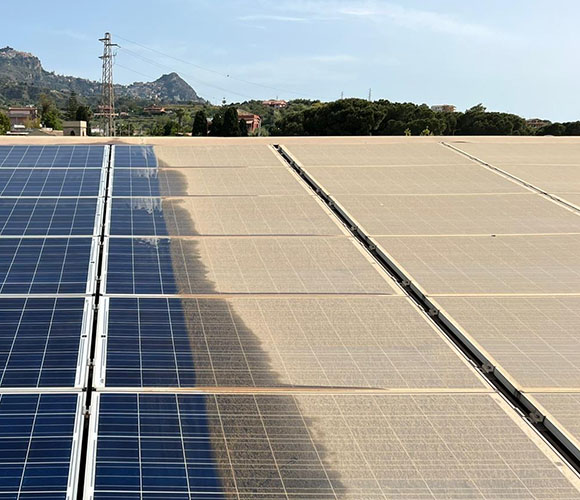
\includegraphics[width=0.5\textwidth]{Images/pannelli_sporchi2.jpg}
	\end{figure}\\
	Per affrontare il problema della pulizia il proprietario dell'impianto può scegliere se rivolgersi ad imprese specializzate che effettuano pulizia a domicilio, oppure prevenire il problema scegliendo di installare pannelli autopulenti di ultima generazione. %lo avevamo detto 
	Entrambe queste soluzioni hanno però dei limiti: per quanto riguarda la prima possibilità, è l'utente stesso che deve accorgersi di quando sopraggiunge il momento opportuno per eseguire la pulizia e deve mobilitarsi per contattare l'impresa adeguata, per un costo che in media varia tra i 100 e i 300\euro.\\
	Parlando invece di pannelli autopulenti essi sono un arma a doppio taglio.\\
	Possono essere realizzati sfruttando diverse tecnologie che spaziano dall'impiego di materiali con attrito estremamente ridotto, sfruttando l'acqua piovana per lavare via la sporcizia, all'uso di impulsi elettrici per far "saltare via" le impurità dalla superficie (recentissima tecnologia dell'MIT non ancora in commercio). Tuttavia, mentre queste tecnologie di ultimissima generazione eccedono la disponibilità economica dei molti, l'uso di materiali dall'attrito ridotto (oltre che prevedere costi di acquisto superiori rispetto ai pannelli tradizionali) comporta una forte dipendenza dalle precipitazioni atmosferiche che possono anche risultare controproducenti, dal momento che in aree cittadine, o generalmente più inquinate, l'acqua piovana andrebbe a depositare ulteriori detriti sulla superficie.\\
	\section{Soluzione proposta}
	La proposta di \emph{Osmos} consiste nel fornire un sistema completamente automatizzato per la pulizia dell'impianto fotovoltaico. L'idea di base è quella di monitorare costantemente l'efficienza energetica di ogni pannello in modo tale da rendersi conto di quando non è più in grado di fornire adeguate prestazioni, a causa dello sporco che vi si è depositato sopra. Quando l'efficienza scende sotto una certa soglia prestabilita dal proprietario il \emph{Osmos} è in grado di effettuare la pulizia usando l'adeguato detergente, reso disponibile in una piccola cisterna installata nello stabile, rilasciandolo sul pannello.\\
	% immagine dell'impianto
	Questa soluzione consentirebbe al proprietario dell'impianto di risparmiare notevolmente sul costo della pulizia e sul tempo da dedicarvi, in quanto il processo avviene automaticamente senza richiedere intervento manuale.\\
	Il liquido adeguato per la pulizia della superficie è l'acqua osmotica, o osmotizzata, che può assere acquistata dall'utente al costo di circa 1 \euro/L in modo che egli possa occuparsi di mantenere attivo il sistema in completa autonomia, senza dover contattare un tecnico o un'impresa specializzata.\\%lo abbiamo detto
	\begin{wrapfloat}{figure}{r}{0pt}
		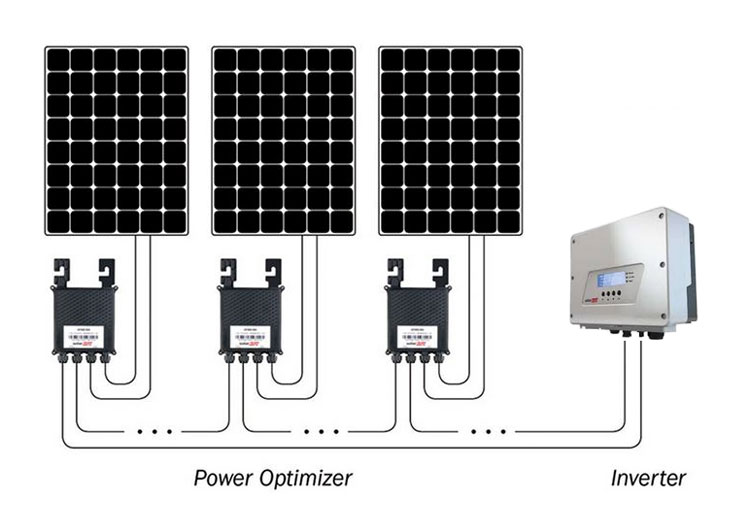
\includegraphics[width=0.5\textwidth]{Images/ottimizzatori.jpg}
	\end{wrapfloat}
	La misurazione dell'efficienza energetica è realizzabile in modo semplice attraverso il dialogo diretto con gli ottimizzatori presenti nell'impianto. Questi dispositivi sono componenti pre-intallate sul retro dei moduli fotovoltaici che, periodicamente, raccolgono i report provenienti dai vari pannelli. Ciascun report contiene, tra le altre informazioni, l'efficienza energetica della quale si può tenere traccia una volta intercettata wireless da \emph{Osmos}. Questo approccio è efficace poiché, invece di sfruttare l'energia prodotta (che può variare a seconda delle condizioni atmosferiche) si basa sull'efficienza, che esprime il rapporto tra l'energia generata e l'energia solare ricevuta. Qualora il valore dovesse diminuire significherebbe che le prestazioni del pannello stanno calando e il sistema si occuperà di rilasciare il detergente sulla superficie.
	\section{Il settore}
	% https://sonnen.it/crescita-del-fotovoltaico-2023-il-boom-e-reale/ --> ho preso tanto da qua
	% https://www.lumi4innovation.it/accumulo-energia-rinnovabili-energy-storage/
	\ emph{Osmos} vuole inserirsi all'interno del settore fotovoltaico, avendo lo scopo di rendere più utili e performanti queste fonti sostenibili.\\\\
	Grazie alla sempre maggiore spinta internazionale verso le fonti di energia rinnovabili, il settore fotovoltaico è in notevole espansione nel mondo.\\
	Importante è anche la crescita della capacità fotovoltaica installata in Italia. Nei primi sette mesi del 2023, in Italia, sono stati installati oltre 2,7 GW, con una crescita del 113\% rispetto allo stesso periodo dell'anno precedente e con un importante contributo degli impianti residenziali (circa il 47\% della capacità totale connessa).\\\\
	Secondo i dati forniti da \href{https://www.terna.it/it/sistema-elettrico/dispacciamento/fonti-rinnovabili}{\emph{Gaudì}}, la potenza fotovoltaica cumulata in Italia, ad agosto 2023, ha superato i 28 GW con oltre 1,4 milioni di installazioni attive. Un dato notevole se si considera che nei primi otto mesi dell'anno sono stati installati 3.123 MW di potenza fotovoltaica con andamenti diversi per i vari segmenti:
	\begin{itemize}
		\item residenziale (impianti sotto i 12 kW) ha registrato l'installazione di 1.379 MW;
		\item commerciale ed industriale (impianti tra i 20 kW e 1 MW) registrati 1.088 MW;
		\item utility-scale (impianti con potenza superiore a 1 MW) aumento di 426 MW.
	\end{itemize}
	I dati registrati dal settore del fotovoltaico e le previsioni di crescita mostrate nelle figure di seguito, sottolineano il ruolo centrale delle fonti rinnovabili nel percorso di transizione energetica globale, riportando un indice CAGR che si aggira intorno al 30\%.
	\begin{center}
		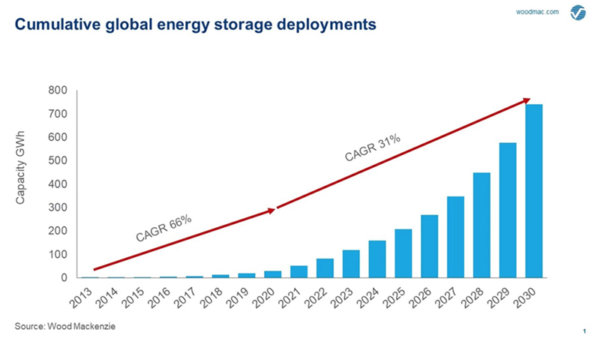
\includegraphics[width=0.7\textwidth]{Images/previsioni_solare.jpg}
		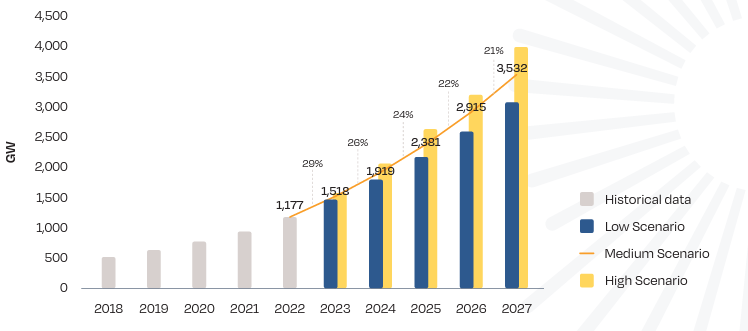
\includegraphics[width=0.7\textwidth]{Images/andamento_pannelli2.png}
	\end{center}
	Il settore del fotovoltaico è sufficientemente vasto da poter essere a sua volta suddiviso in due parti: una prima parte che comprende le imprese produttrici di moduli fotovoltaici (in cui i principali attori sono \emph{Sunpower, Panasonic, Exe Solar} e simili) e una seconda parte che riguarda le imprese produttrici di componenti cooperanti coi moduli fotovoltaici.\\\\
	Sebbene esistano enti che si pongono a cavallo di questa partizione, \emph{Osmos} fa capo solamente alla seconda categoria. All'interno di questa non vi è grande frammentazione, infatti la maggioranza è occupata da \emph{Abb Spa}: una società fortemente coinvolta nella produzione di apparecchiature che garantiscono continuità di servizio, affidabilità e ritorno dell'investimento tramite interruttori, dispositivi di misurazione, sensori e altro.\\
	I prodotti e servizi forniti da \emph{Abb Spa} sono poi utilizzabili anche in moltissimi altri settori eterogenei; questo aumenta considerevolmente l'influenza e il potere economico dell'impresa stessa, dandole la possibilità di imporsi nei confronti di altre società più specializzate quali \emph{Enel X} e \emph{SoralEdge Tecnology} come riportato nel grafico seguente:\\
	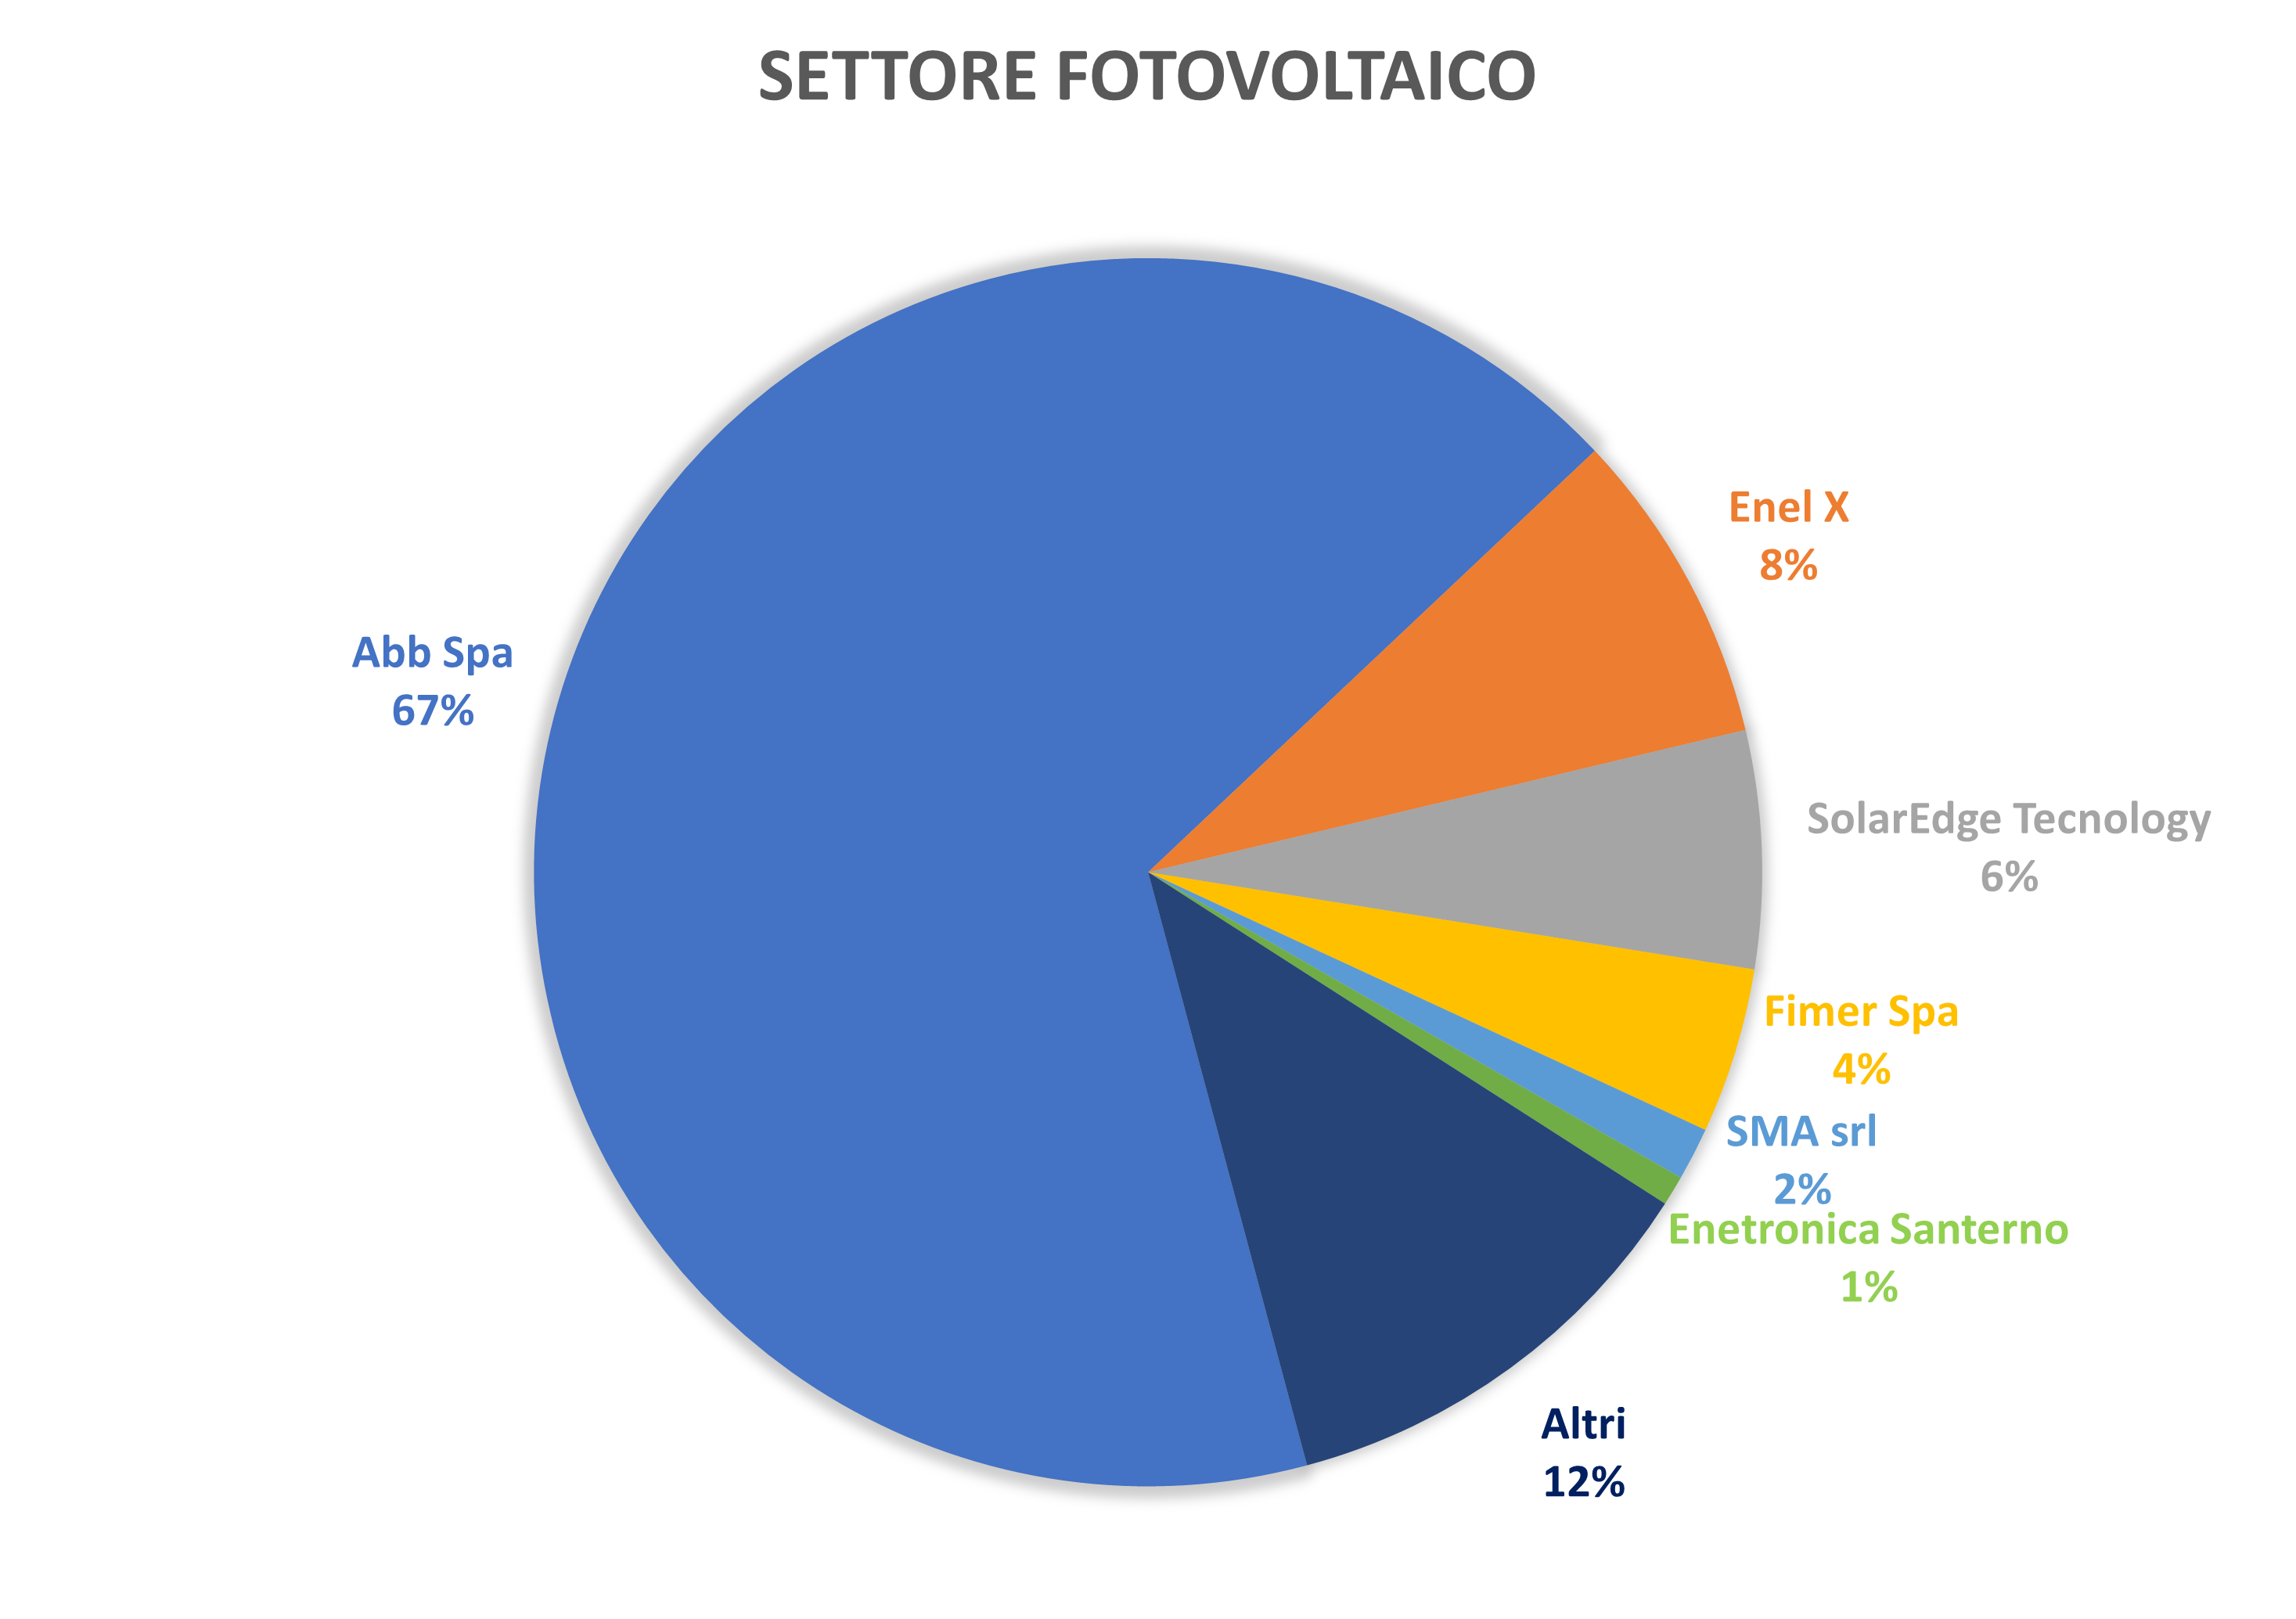
\includegraphics[width=\textwidth]{Images/suddivisione_settore.png}
	La proposta di \emph{Osmos} è ritenuta interessante per l'attuale situazione del settore, sia perché l'ambito del fotovoltaico si sta ampliando, sia a causa della mancanza di una soluzione a supporto dei moduli fotovoltaici specializzata nella pulizia di questi, ad esclusione dei pannelli autopulenti già menzionati.\\
	La strategia adottata è riportata di seguito:
	\begin{center}
		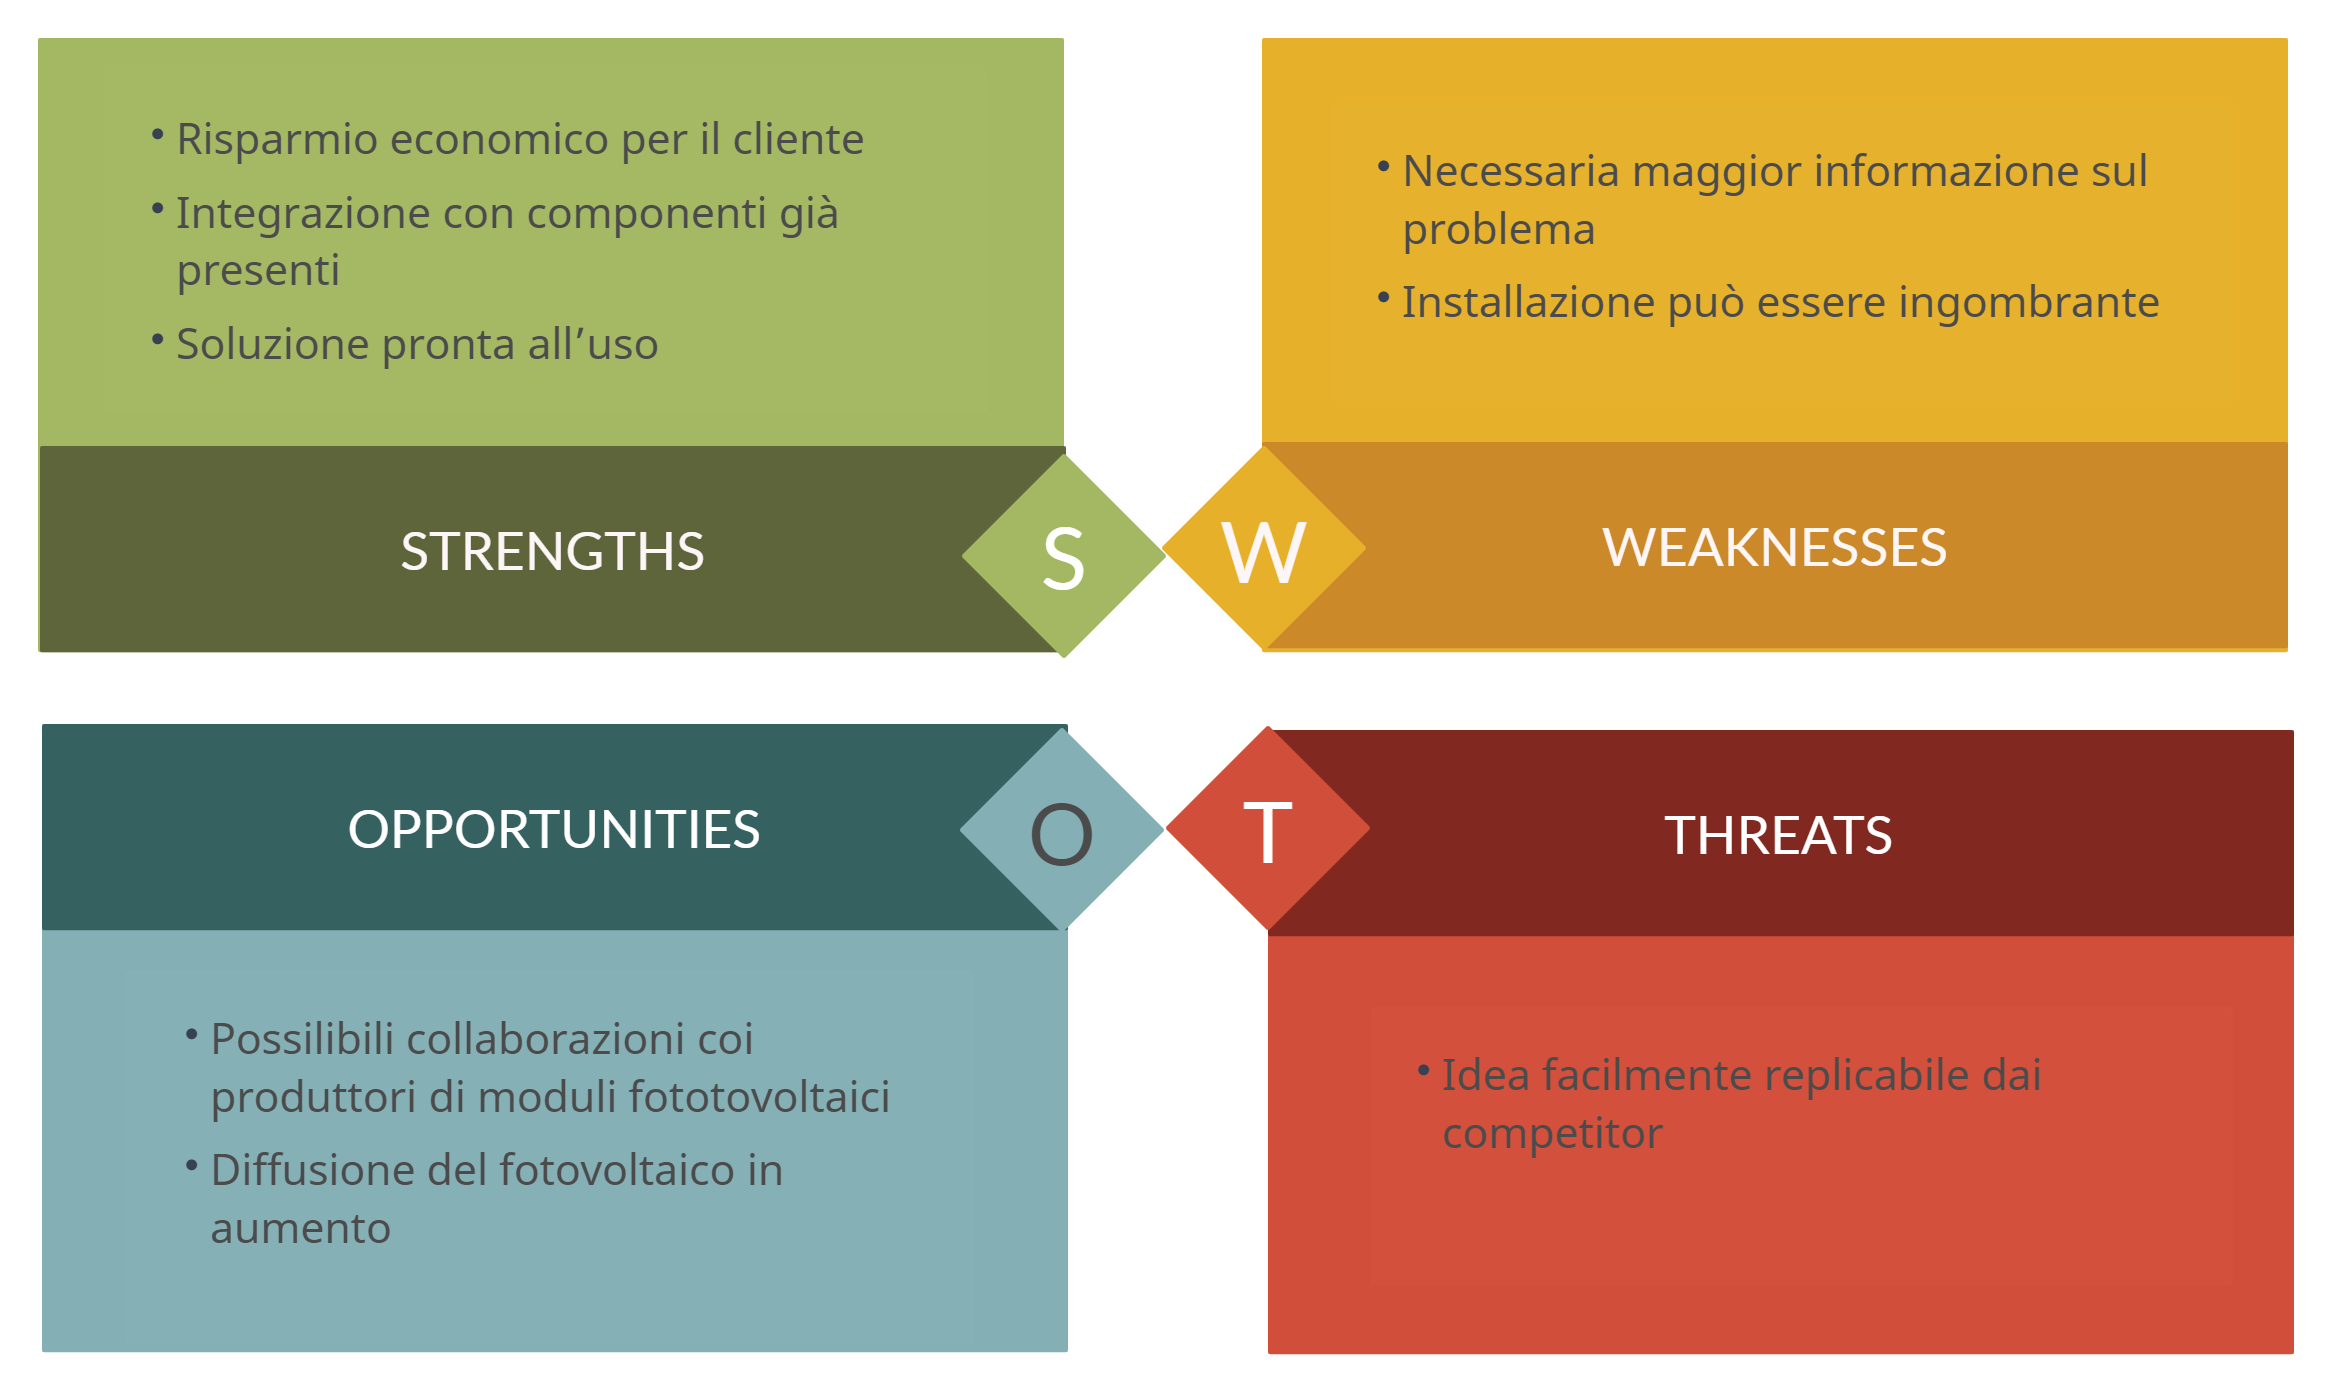
\includegraphics[width=0.9\textwidth]{Images/SWOT2.png}
	\end{center}
	Inoltre, si riportano qui gli obiettivi perseguiti da \emph{Osmos} confrontati con quelli dei principali competitor sopra citati:
	\begin{center}
		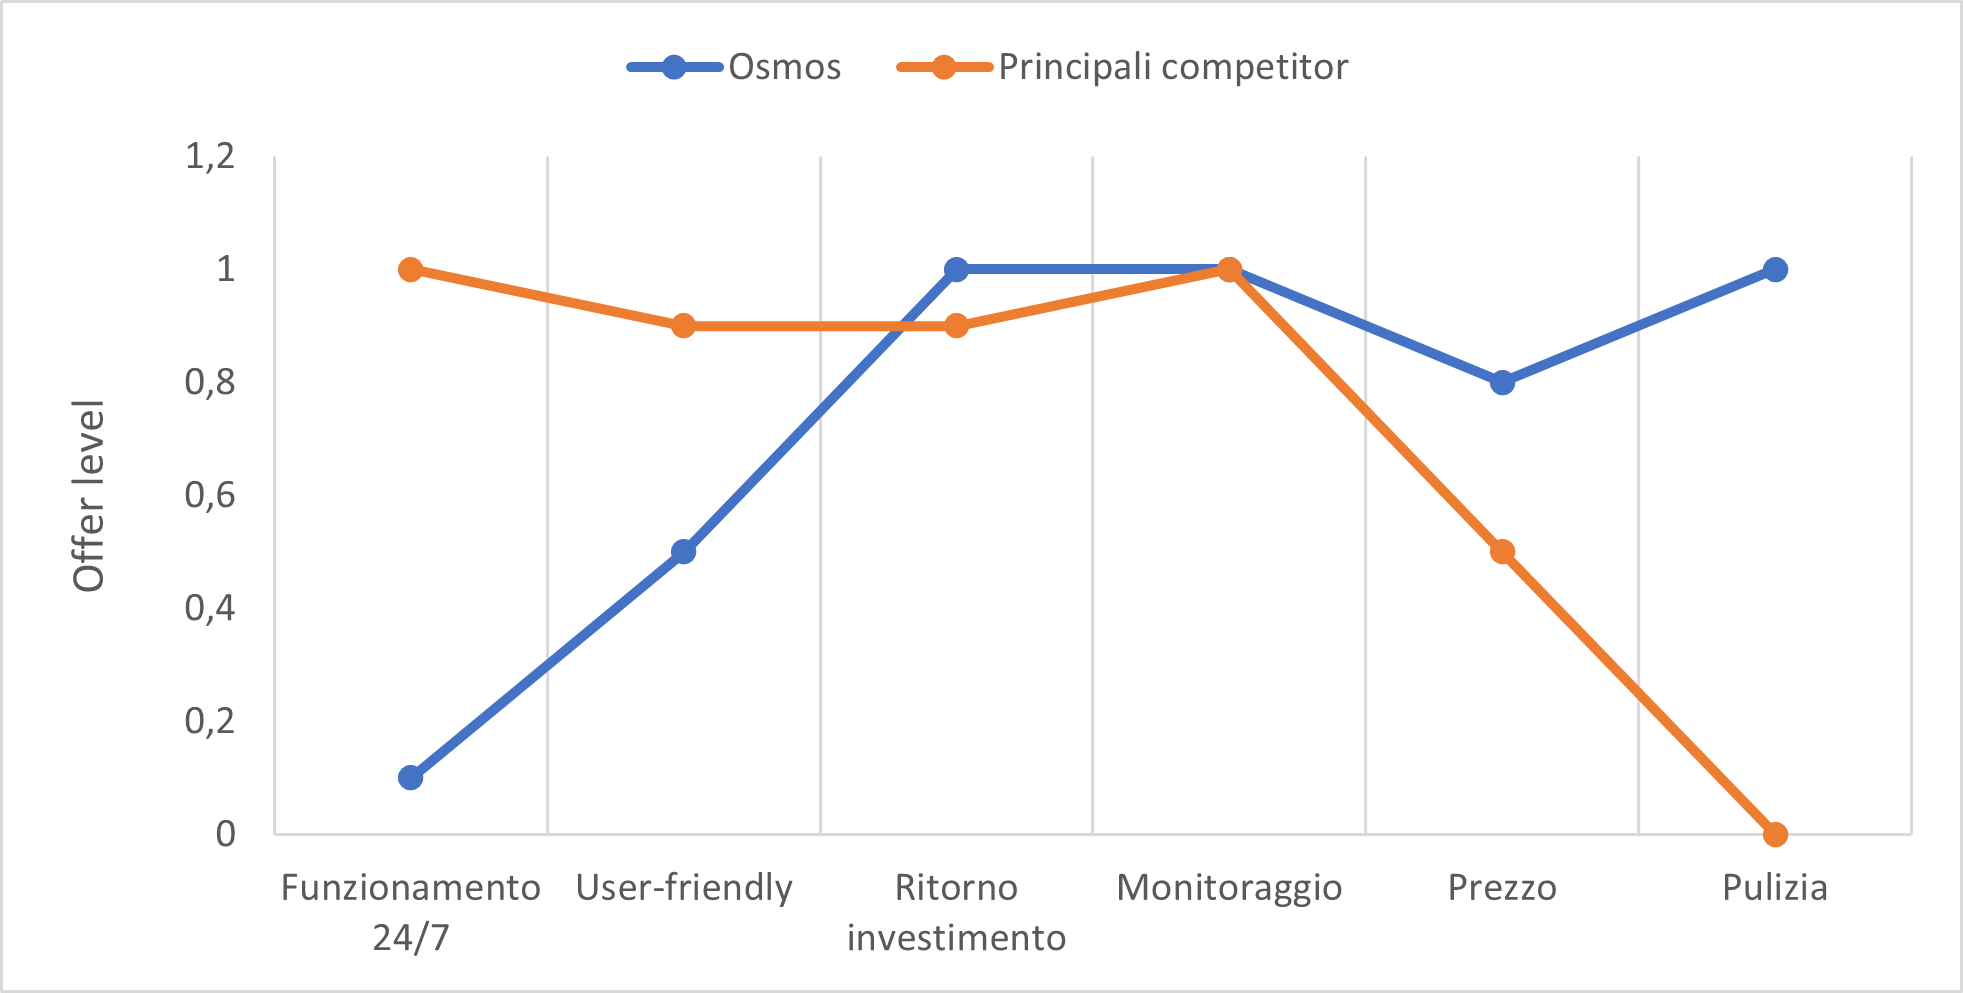
\includegraphics[width=\textwidth]{Images/curve_valore.png}
	\end{center}
	Tra queste caratteristiche spiccano in particolar modo il funzionamento 24/7 e l'offerta di un prodotto user-friendly. Il nostro prodotto non ha bisogno di essere costantemente in funzione, ma necessita di essere operativo solamente in quei pochi minuti del giorno che comprendono l'analisi delle prestazioni ed eventualmente l'esecuzione della pulizia.\\
	Per quanto invece riguarda la possibilità di offrire un prodotto user-friendly, questa non è una caratteristica fondamentale per \emph{Osmos}, in quanto alla base del prodotto stesso vi è l'idea di minimizzare l'interazione con l'utente, facendo in modo che il sistema operi in modo invisibile agli occhi del cliente.
	\section{Il mercato e il cliente}
	\emph{Osmos} è un prodotto pensato per essere commercializzato ad un pubblico composto tanto da utenti privati possessori di impianti domestici, quanto da titolari di aziende che fanno uso di impianti su scala maggiore (B2C).\\
	Tuttavia non si esclude la possibilità di stipulare contratti specifici con imprese produttrici e/o installatrici di moduli fotovoltaici (B2B). Queste potrebbero desiderare di fornire ai loro clienti impianti fotovoltaici già dotati dei un sistema di pulizia come prodotti all-in-one. A tal proposito, si potrebbe pianificare la vendita di grandi lotti di sistemi \emph{Osmos} a queste imprese.\\\\
	Per studiare i bisogni e i desideri dei potenziali clienti si è deciso di diffondere un survey contenente domande di vario genere legate ai pannelli fotovoltaici, diversificate in base a possessori o non possessori dei suddetti. Nei confronti dei primi è stata posta particolare attenzione al tema della pulizia.\\
	A valle di diverse centinaia di risposte basate su un campione il più eterogeneo possibile, si sono osservati dati particolarmente interessanti: per quanto riguarda individui che già possiedono dispositivi fotovoltaici si è notato non solo che oltre la metà di essi attribuiscono massima importanza all'efficienza energetica, ma anche che circa il 46\% degli utenti ha evidenziato un importante calo delle prestazioni nel tempo.\\
	Inoltre è emerso come il prezzo pagato per la pulizia (compreso in media tra 100 e 150\euro) sia considerato eccessivo da molti.
	\begin{center}
		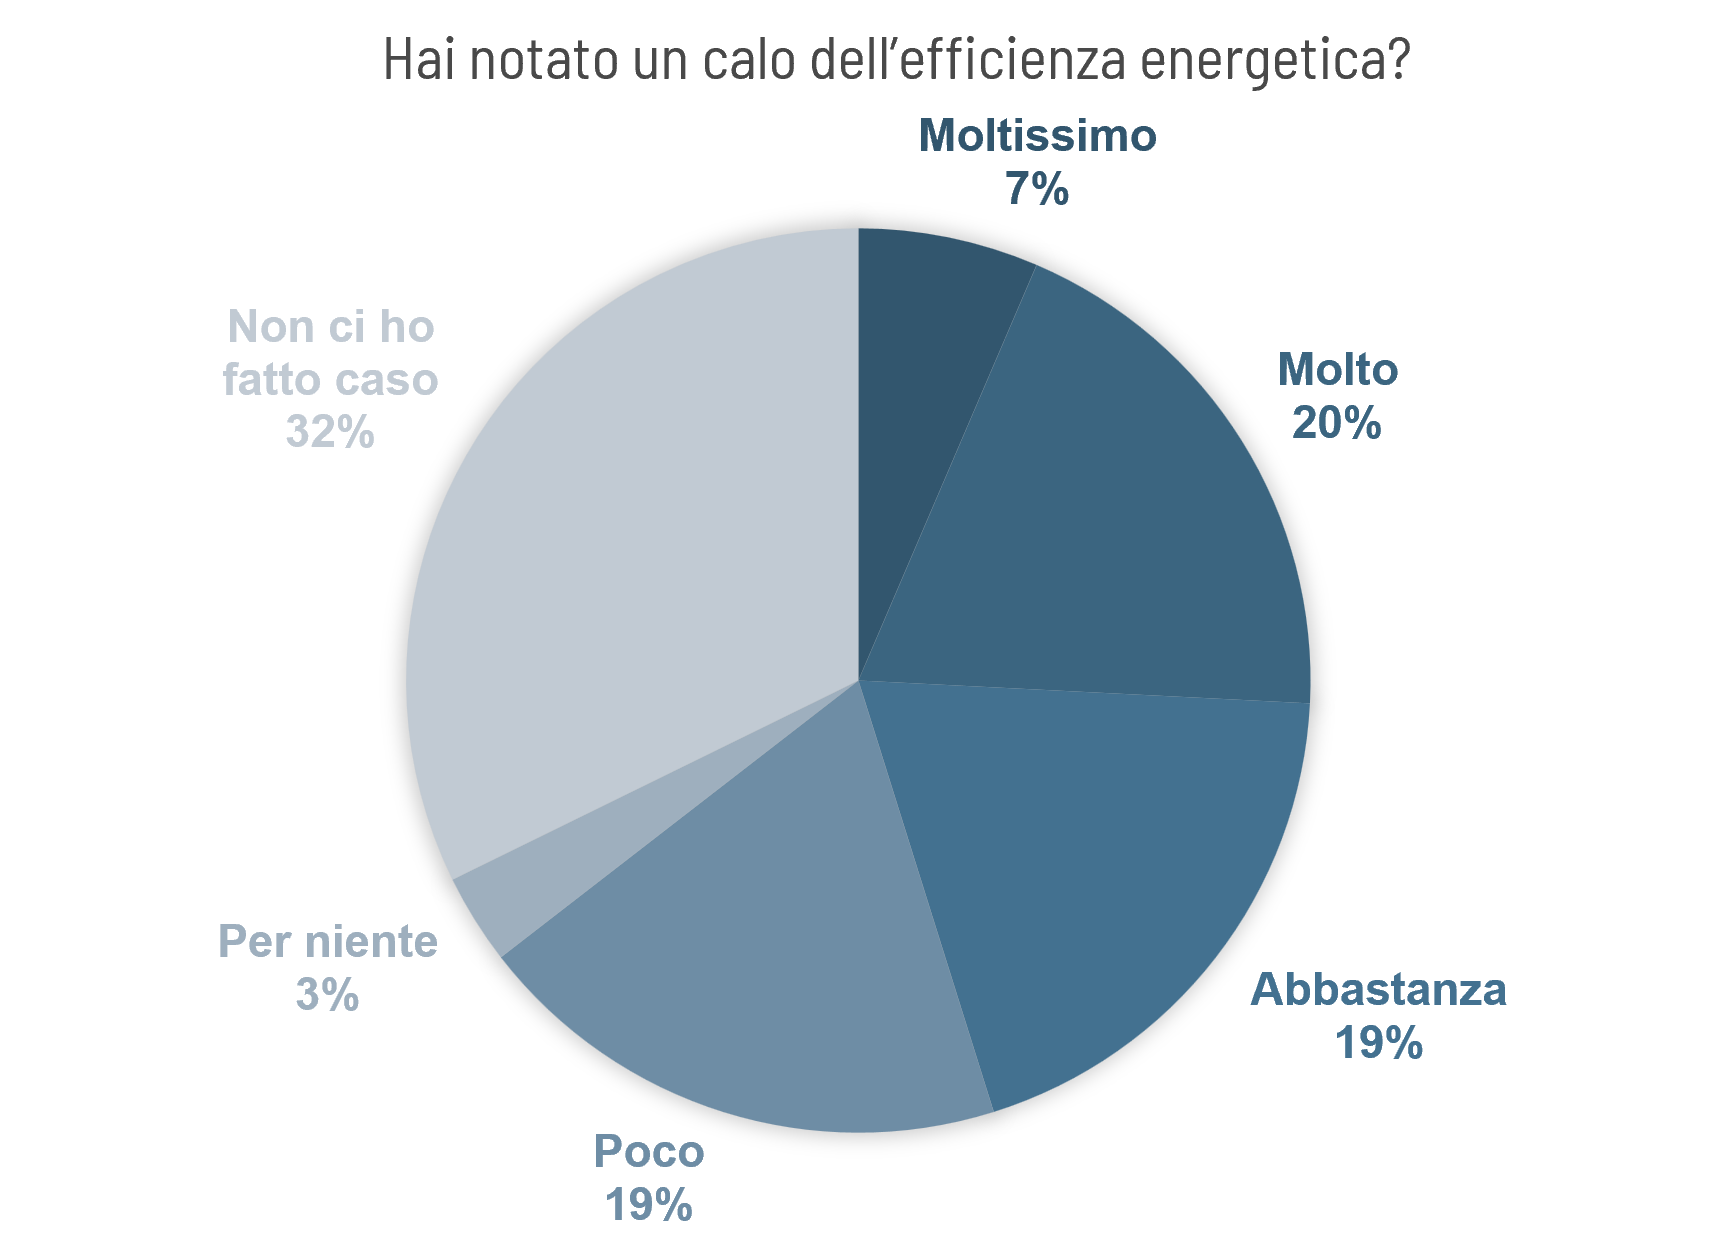
\includegraphics[width=0.45\textwidth]{Images/effetti_efficienza.png}
		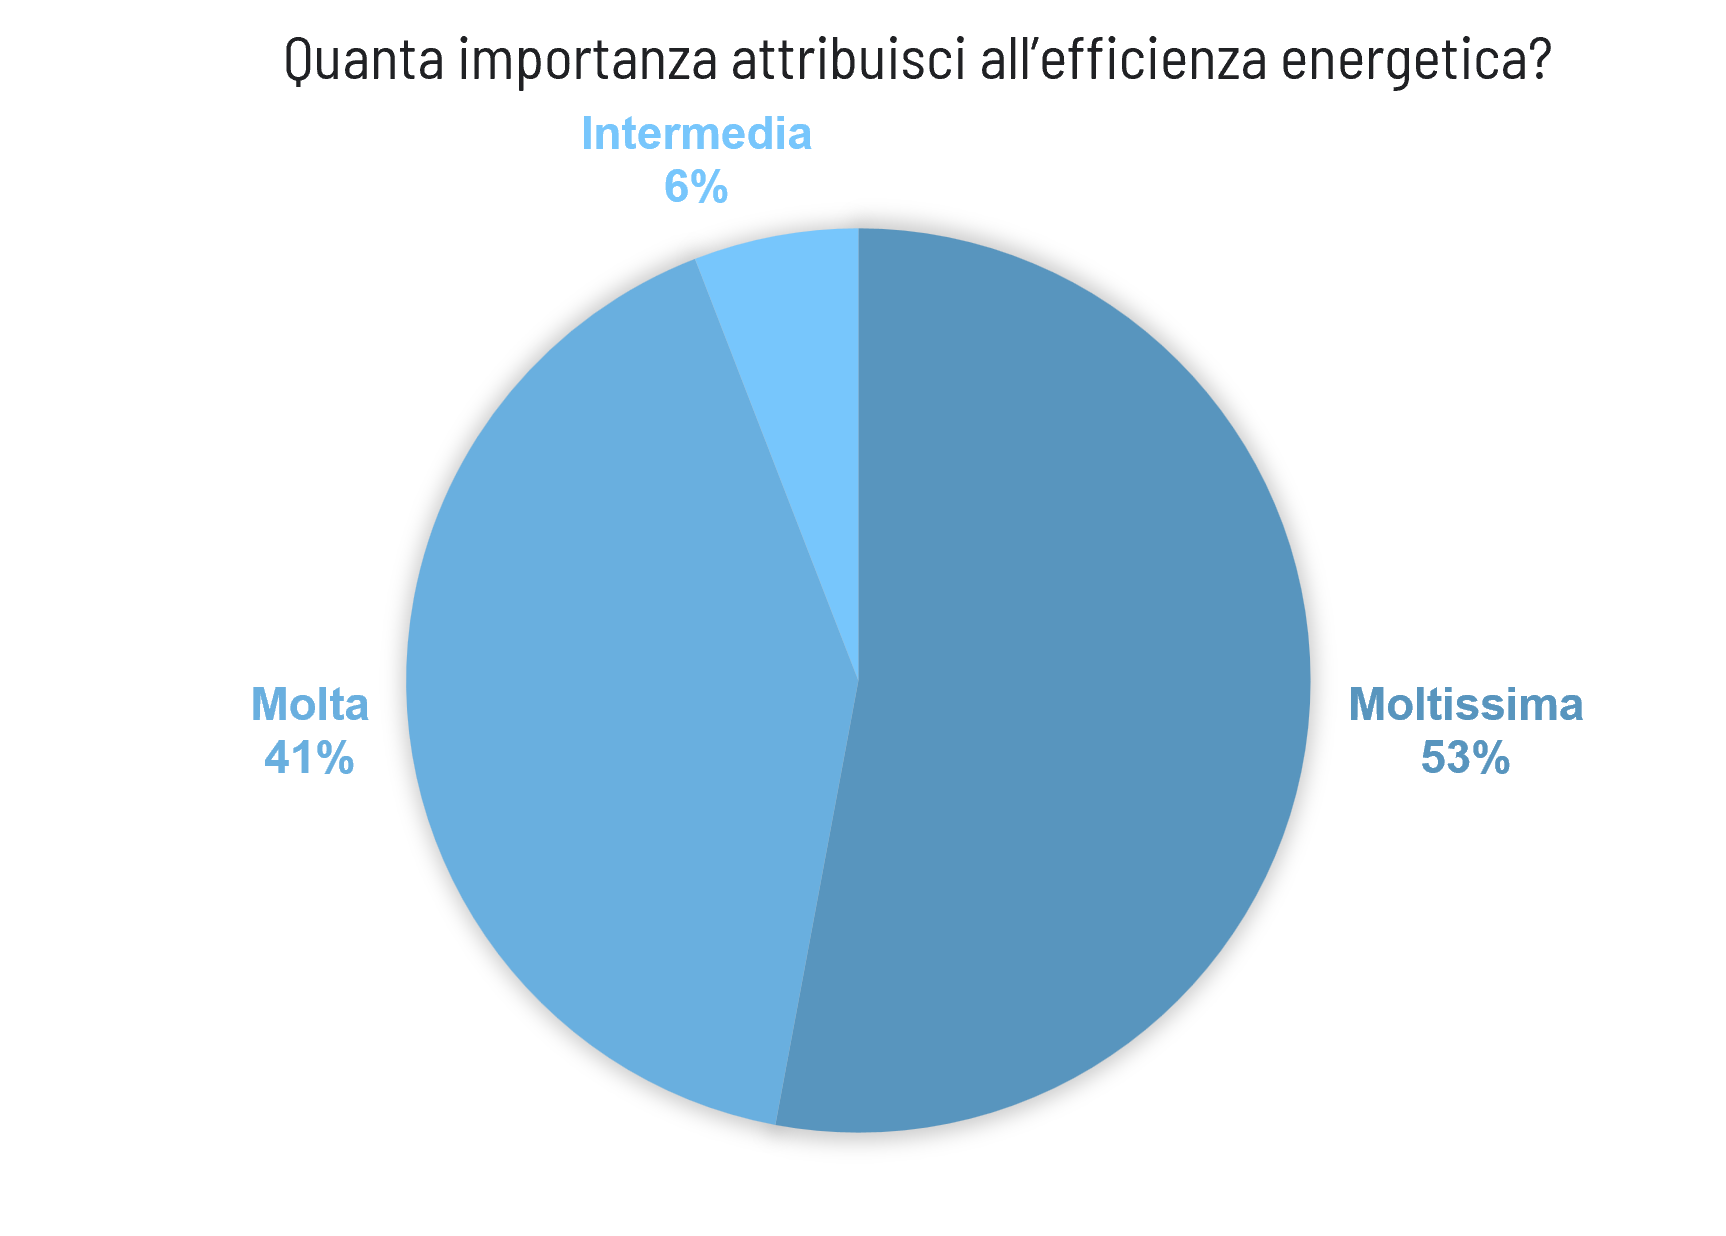
\includegraphics[width=0.45\textwidth]{Images/importanza_efficienza.png}
	\end{center}
	Analizzando invece i dati forniti da individui che non possiedono impianti fotovoltaici si è potuto dedurre che essi non usufruiscono del prodotto non perché non ne siano interessati ma per altre motivazioni: circa 3 persone su 4 riferiscono che il costo di acquisto è eccessivo (35.7\%) oppure risiedono in un edificio non di proprietà (39.9\%). A rafforzare questo dato vi è anche il fatto che la quasi totalità del campione che non possiede impianti fotovoltaici è comunque convinta che questi forniscano benefici economici.
	\begin{center}
		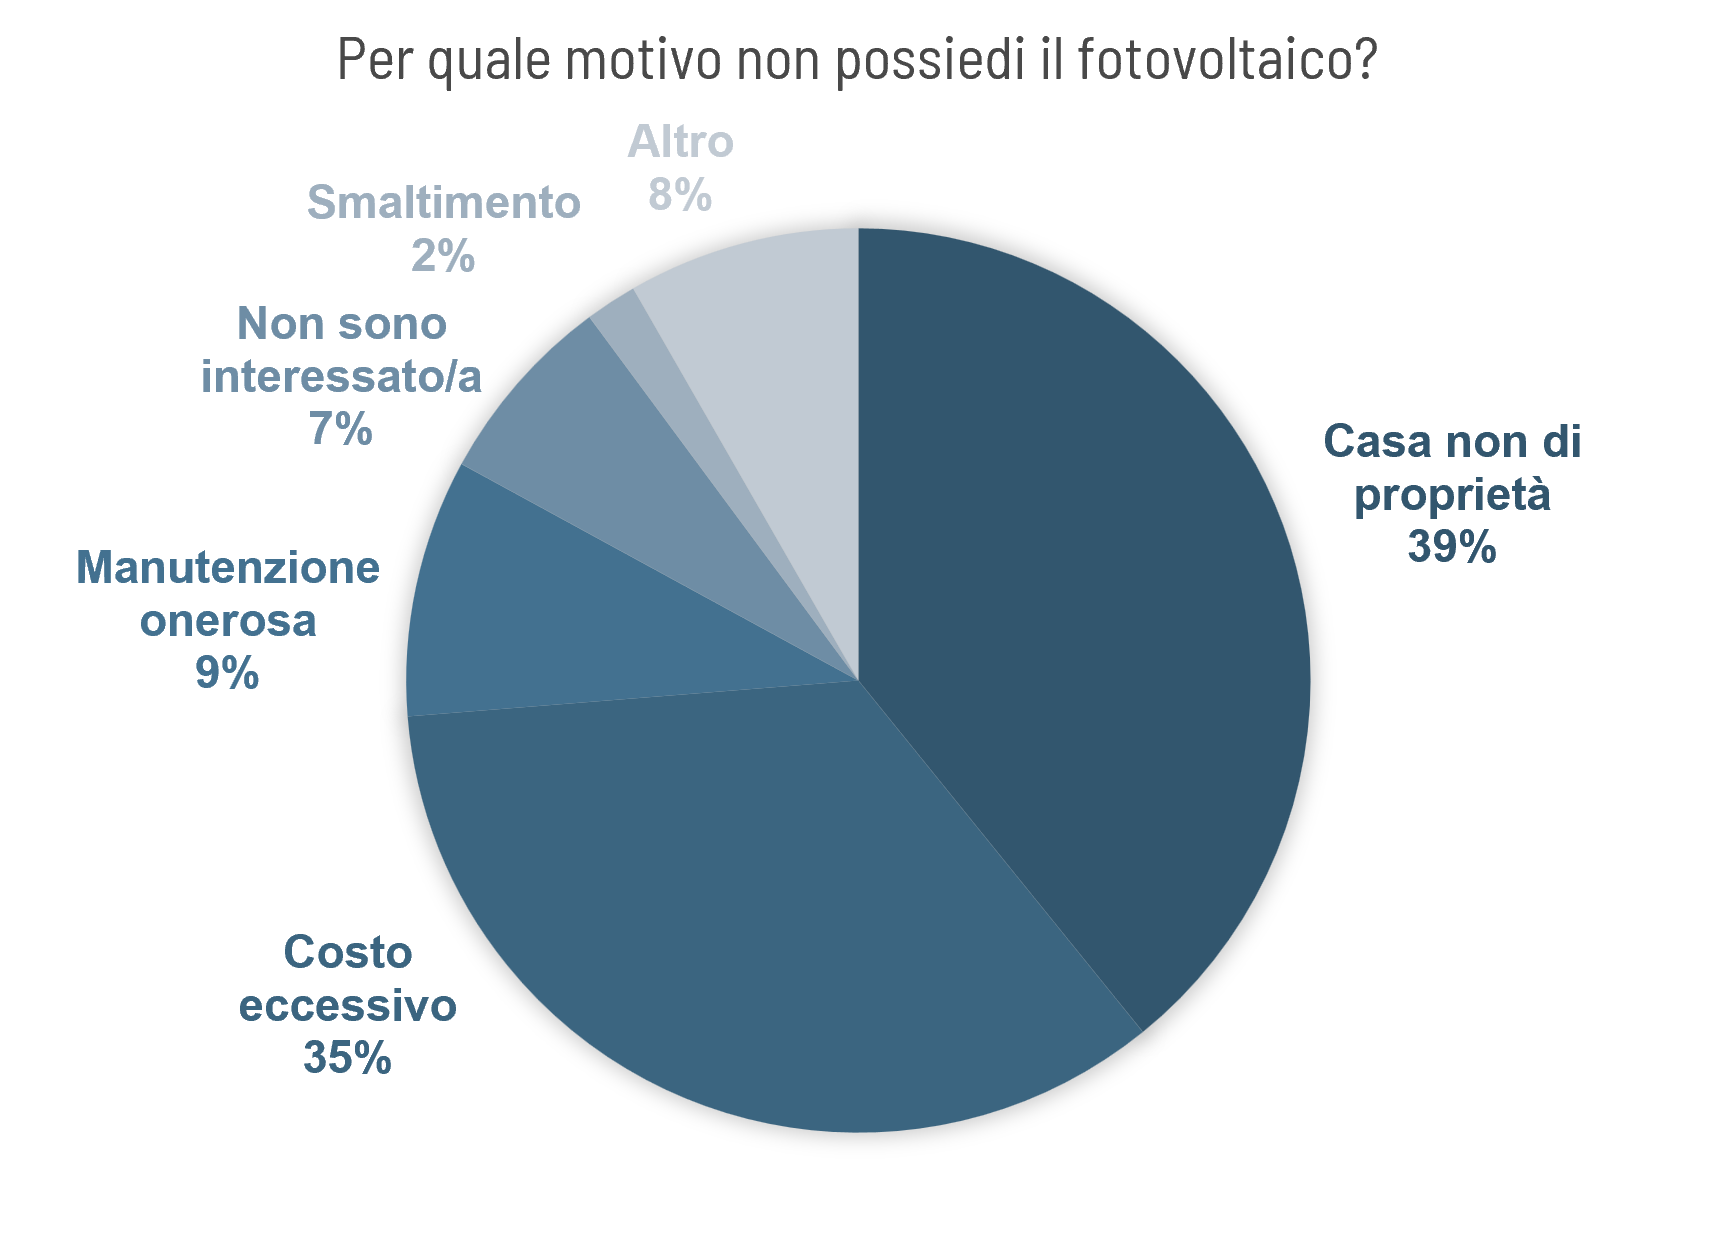
\includegraphics[width=0.45\textwidth]{Images/no_pannelli.png}
		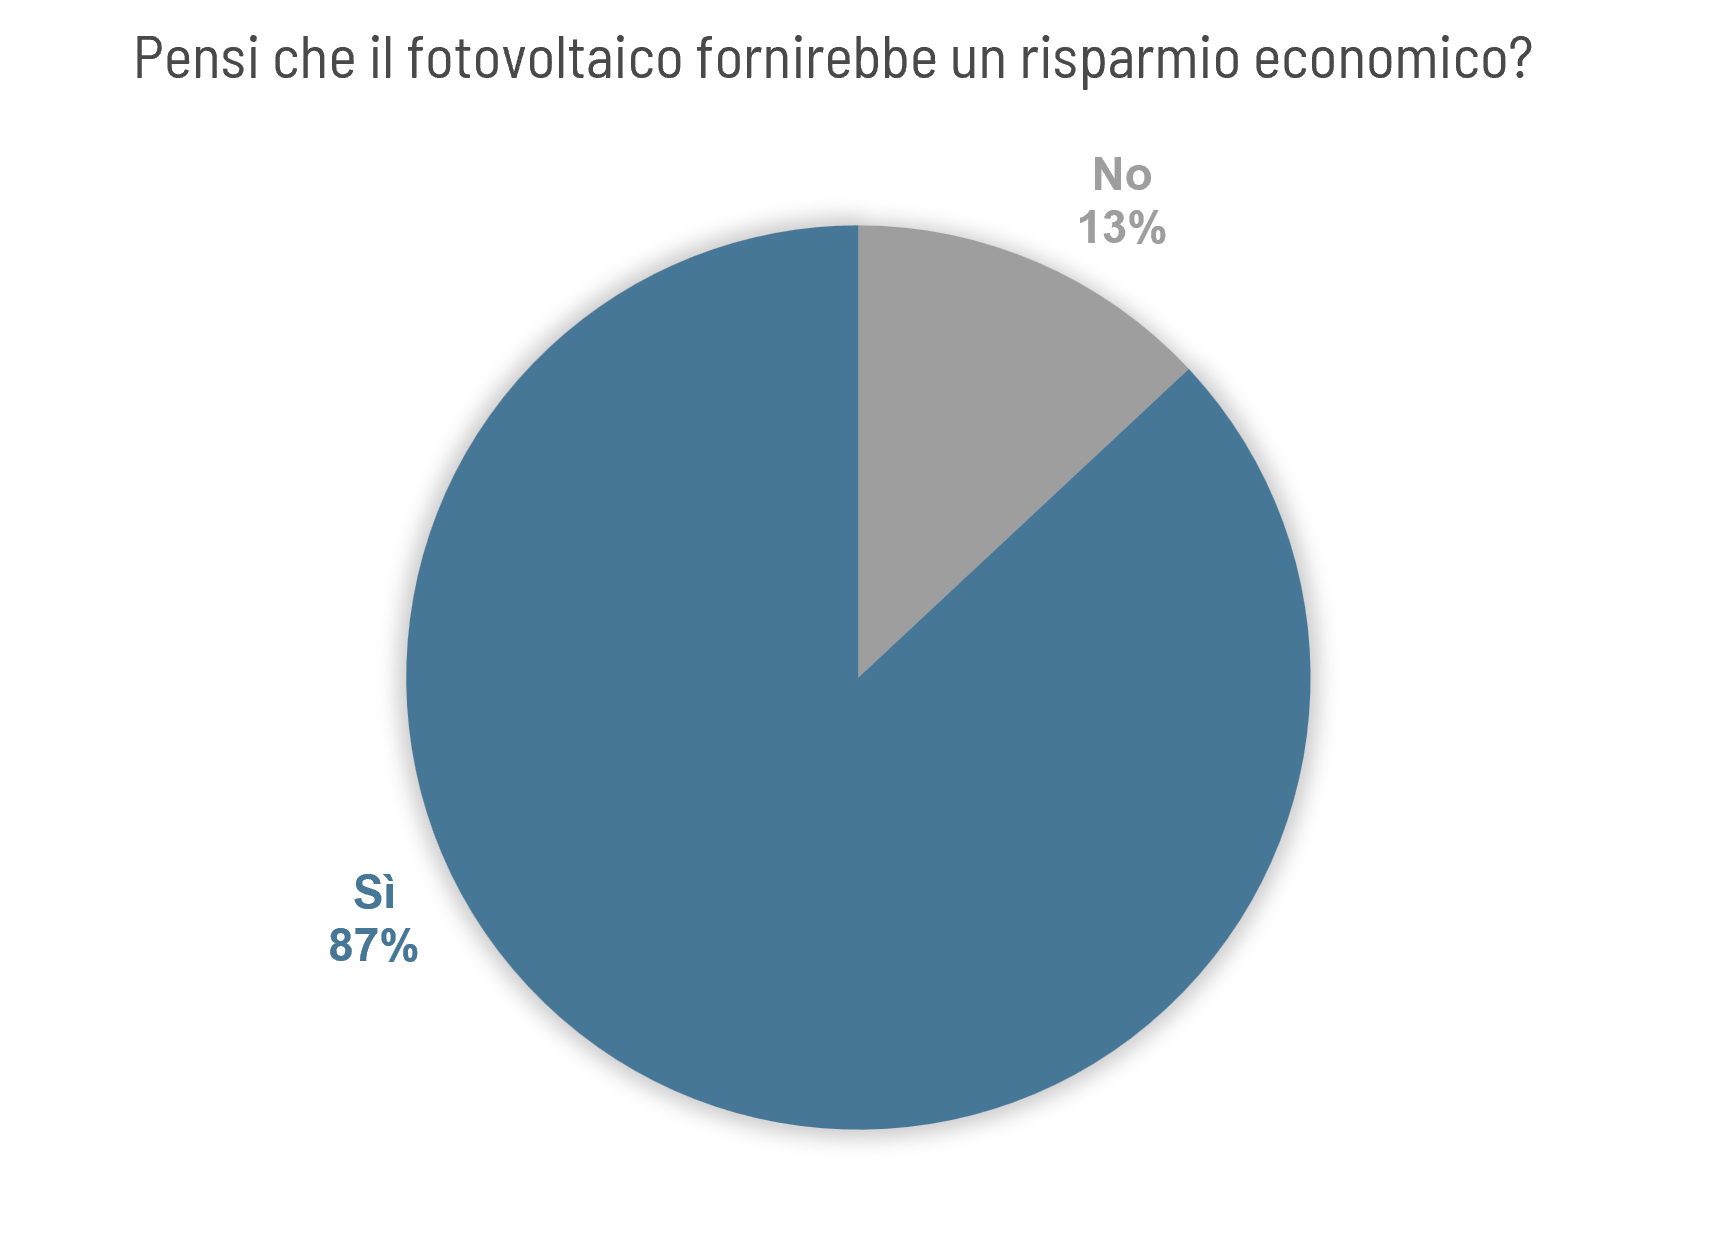
\includegraphics[width=0.45\textwidth]{Images/vantaggi_pannelli.png}
	\end{center}
	A seguito dell'indagine di mercato svolta tramite la survey si sono utilizzati tutti i dati ricavati combinandoli per realizzare il profilo del cliente medio coinvolto nel settore di riferimento allo scopo di identificare i bisogni, i desideri e le paure dei potenziali clienti. Tutto ciò è riportato nel seguente schema:
	\begin{center}
		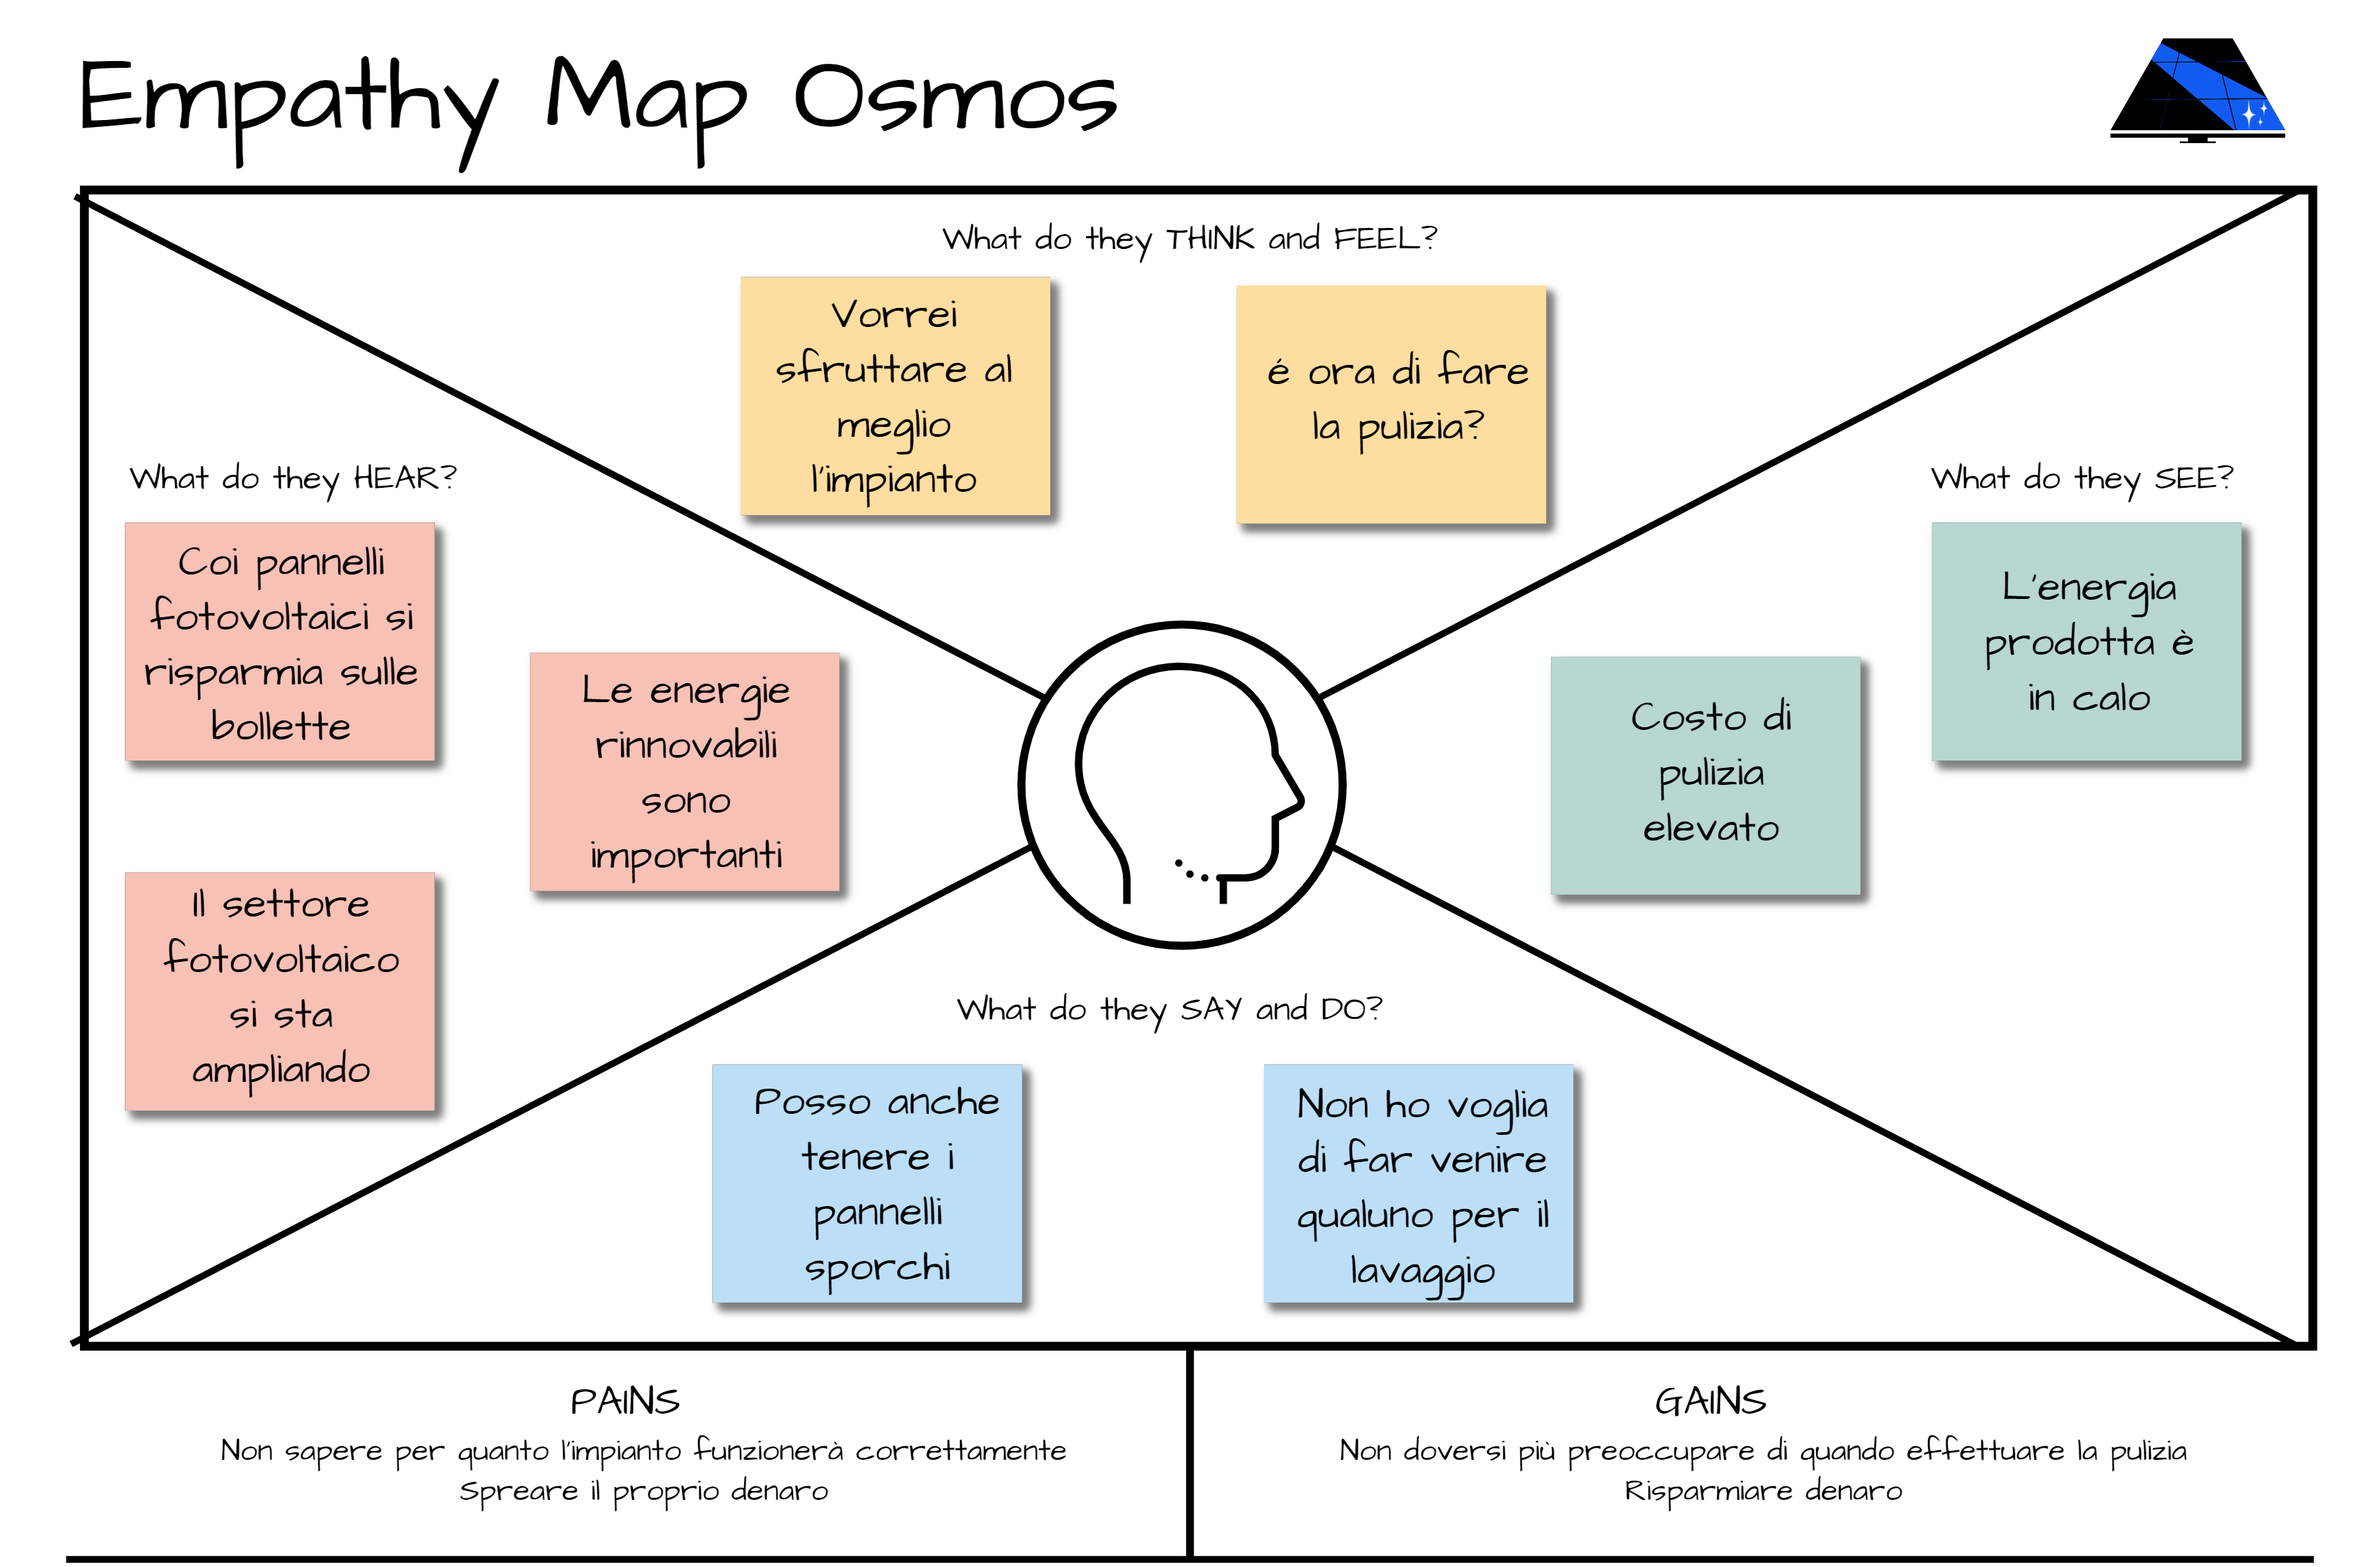
\includegraphics[width=0.9\textwidth]{Images/EmpathyMap.png}
	\end{center}
	Una volta individuati i bisogni del pubblico è necessario procedere a classificarli singolarmente, differenziando quelli che il cliente considera come di massima importanza da quei bisogni ritenuti secondari o trascurabili.\\
	In questo modo ogni bisogno (o caratteristica del prodotto finale) è stato classificato come appartenente ad una gerarchia composta da 4 categorie: \emph{Must} (ciò che la soluzione finale deve soddisfare a tutti i costi), \emph{Should} (elementi ad alta priorità da includere subito dopo i precedenti), \emph{Could} (requisiti auspicabili, inseriti se tempo e risorse lo permettono) e \emph{Won't} (caratteristiche che accetto di non vedere implementate ma che posso considerare in futuro)
	\begin{center}
		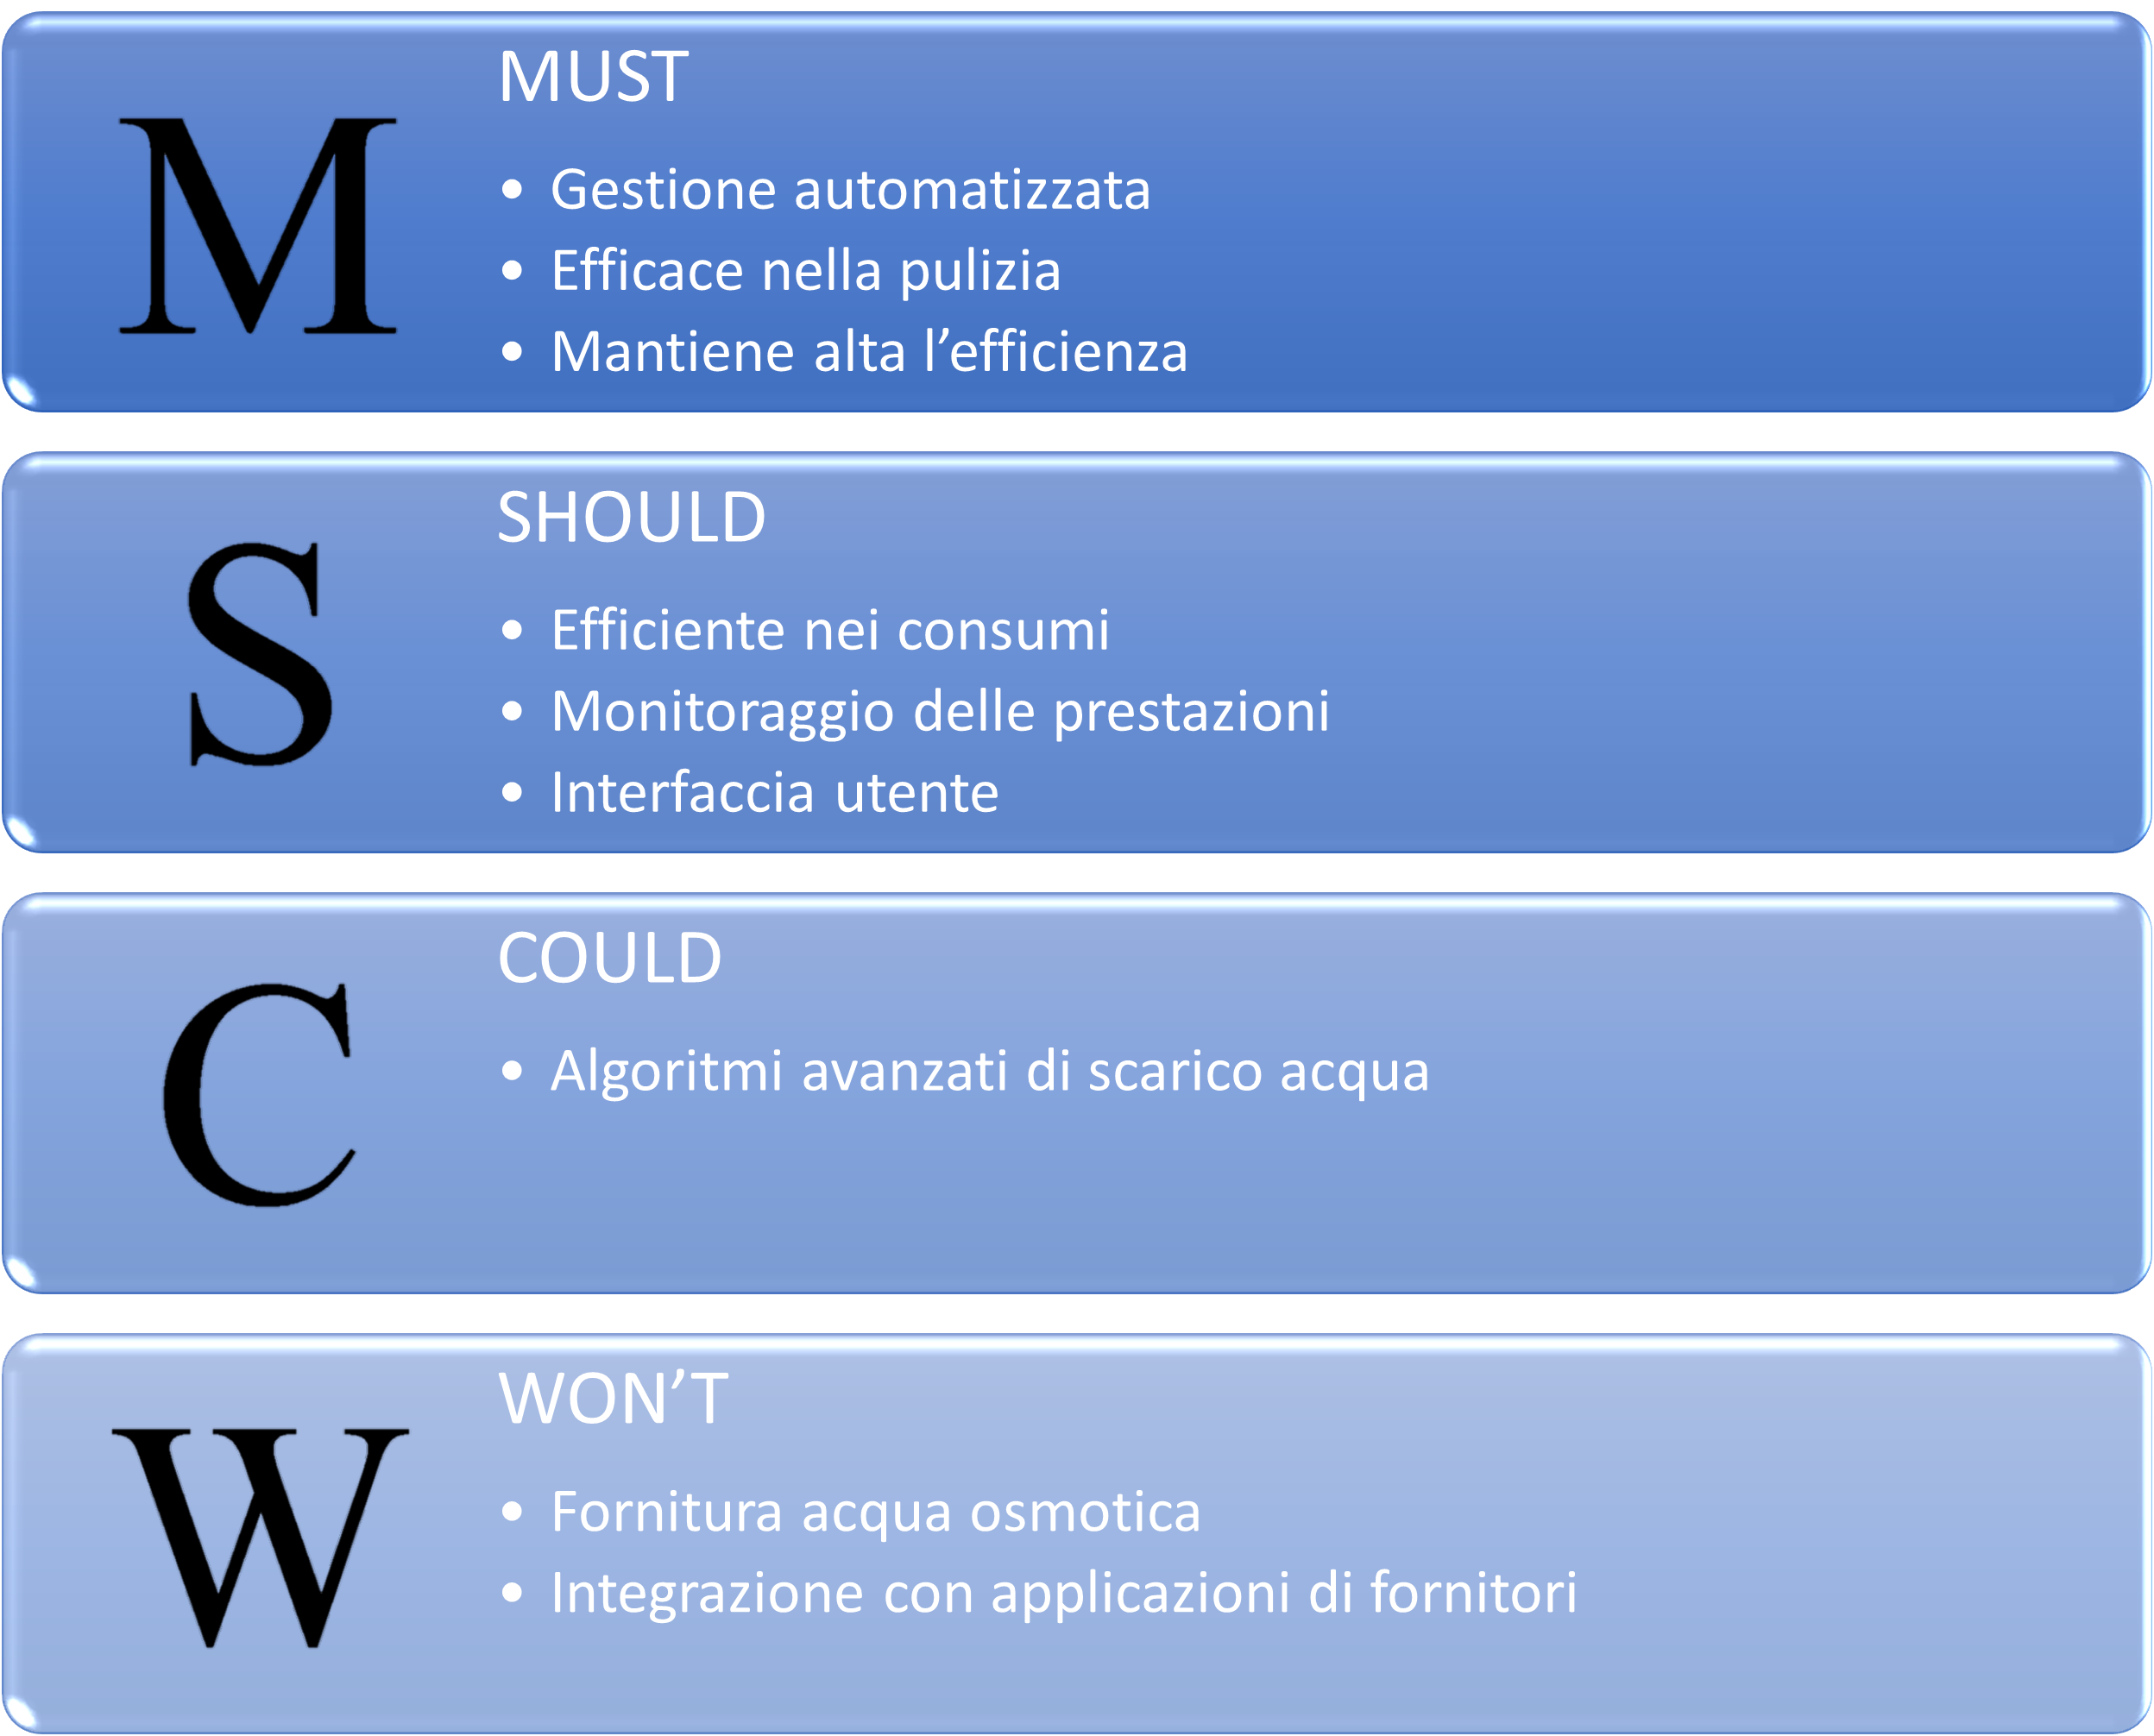
\includegraphics[width=0.6\textwidth]{Images/MoSCoW.png}
	\end{center}
	\section{Modello di business}
	\textbf{Value Proposition}\\
	L'obiettivo di \emph{Osmos} è fornire e installare sistemi per la pulizia automatica dei moduli fotovoltaici. Questi sistemi sono indirizzati sia agli utenti privati, possessori di impianti domestici, sia verso imprese che possiedono una superficie fotovoltaica notevolmente superiore. %già detto credo 2 volte almeno
	I sistemi proposti forniscono ai clienti non solo la possibilità di sfruttare impianti che mantengono un alto livello di efficienza energetica ma anche di risparmiare sul costo della pulizia, dal momento che non ci sarà più la necessità di rivolgersi ad una ditta esterna per eseguirla. Così facendo il cliente dovrebbe unicamente occuparsi di rifornirsi di acqua osmotica per riempire il relativo serbatoio con cui poi il sistema effettua la pulizia.\\
	Inoltre \emph{Osmos} risulterà essere una naturale estensione dell'impianto fotovoltaico già installato dato che non entra in conflitto ma coopera con le componenti già presenti. Ciò garantisce un'installazione che non va in alcun modo a compromettere le caratteristiche e componenti dell'impianto già presente.\\\\
	\textbf{Relazione col cliente}\\
	Il primo contatto con il cliente può essere stabilito tramite la stessa impresa produttrice e installatrice dell'impianto fotovoltaico, che informa della possibile installazione anche di un sistema \emph{Osmos}, oppure tramite spot pubblicitari online attraverso social network e pubblicità mirata. In questo modo diventa possibile intercettare anche consumatori entranti nel settore sempre crescente, rendendoli consci del problema fin dal momento dell'acquisto dei pannelli.\\
	Una volta entrati in contatto con l'acquirente, dopo l'avvenuta installazione si ha l'obiettivo di mantenere il rapporto col cliente tramite la fornitura di un servizio di assistenza disponibile per via telefonica, utilizzabile dall'utente per contattare l'assistenza in caso di malfunzionamenti del sistema o problemi di qualsiasi genere legati ad esso, di modo da poter intervenire tempestivamente.\\\\
	\textbf{Elementi chiave}\\
	\emph{Osmos} attribuisce molto peso all'esecuzione di un sopralluogo del sito di installazione per essere in grado di pianificare la soluzione che meglio si adatta al singolo cliente.\\
	Una volta avvenuta l'installazione risulta di vitale importanza un adeguato monitoraggio dell'efficienza energetica nel tempo, reso possibile dalla storyline dell'impianto fotovoltaico. Questa garantisce l'avvio della pulizia nel momento ideale allo scopo di attestare le prestazioni su valori elevati e di prolungare la vita del modulo fotovoltaico.\\
	Notevole importanza è poi attribuita anche ai partner. Come visto in precedenza, si ha intenzione di instaurare un legame con un'impresa fornitrice di impianti fotovoltaici. Questo garantirebbe non solo una più facile divulgazione dell'importanza della pulizia dei pannelli, ma andrebbe anche a favorire un aumento del numero di clienti entranti nel settore.\\
	Inoltre, avendo la possibilità di stipulare contratti con le imprese fornitrici di materie prime (quali microcontrollori hardware per l'implementazione della logica e componenti idraulici), si andrebbero a ridurre i costi di produzione, aumentando di conseguenza il margine di profitto.\\\\
	% idee:
	%	- adeguata pianificazione dell'installazione nel domicilio: soluzione applicata ad hoc per il cliente (attività)
	%	- collaborazione con impresa che installa pannelli (partner chiave) grazie ad essa si facilità la divulgazione del prblema che andiamo a risolvere
	%	- forniori di materie prime sia Arduino che a livello idraulico (partner)
	\textbf{Analisi costi e ricavi}\\
	In Italia, il costo medio per effettuare una pulizia completa dell'impianto si aggira tra i 100 e i 300\euro: un costo che varia a seconda della condizione in cui versano i pannelli, della posizione nella quale questi sono installati e dalle dimensioni della superficie. \emph{Osmos} punta a fornire un prodotto dal costo complessivo e indicativo per il cliente finale di 500\euro: un prezzo dato in gran parte dalla manodopera in fase di installazione ma variabile proprio in base a questa.\\
	Il costo delle materie prime è invece più limitato: oltre al software necessario (di nostra produzione) è richiesto solamente un microcontrollore e le componenti idrauliche necessarie al rilascio di acqua osmotica, per un costo totale stimato di 120\euro.\\
	L'obiettivo risulta quello di ottenere un profitto del 20\% su ogni installazione.\\
	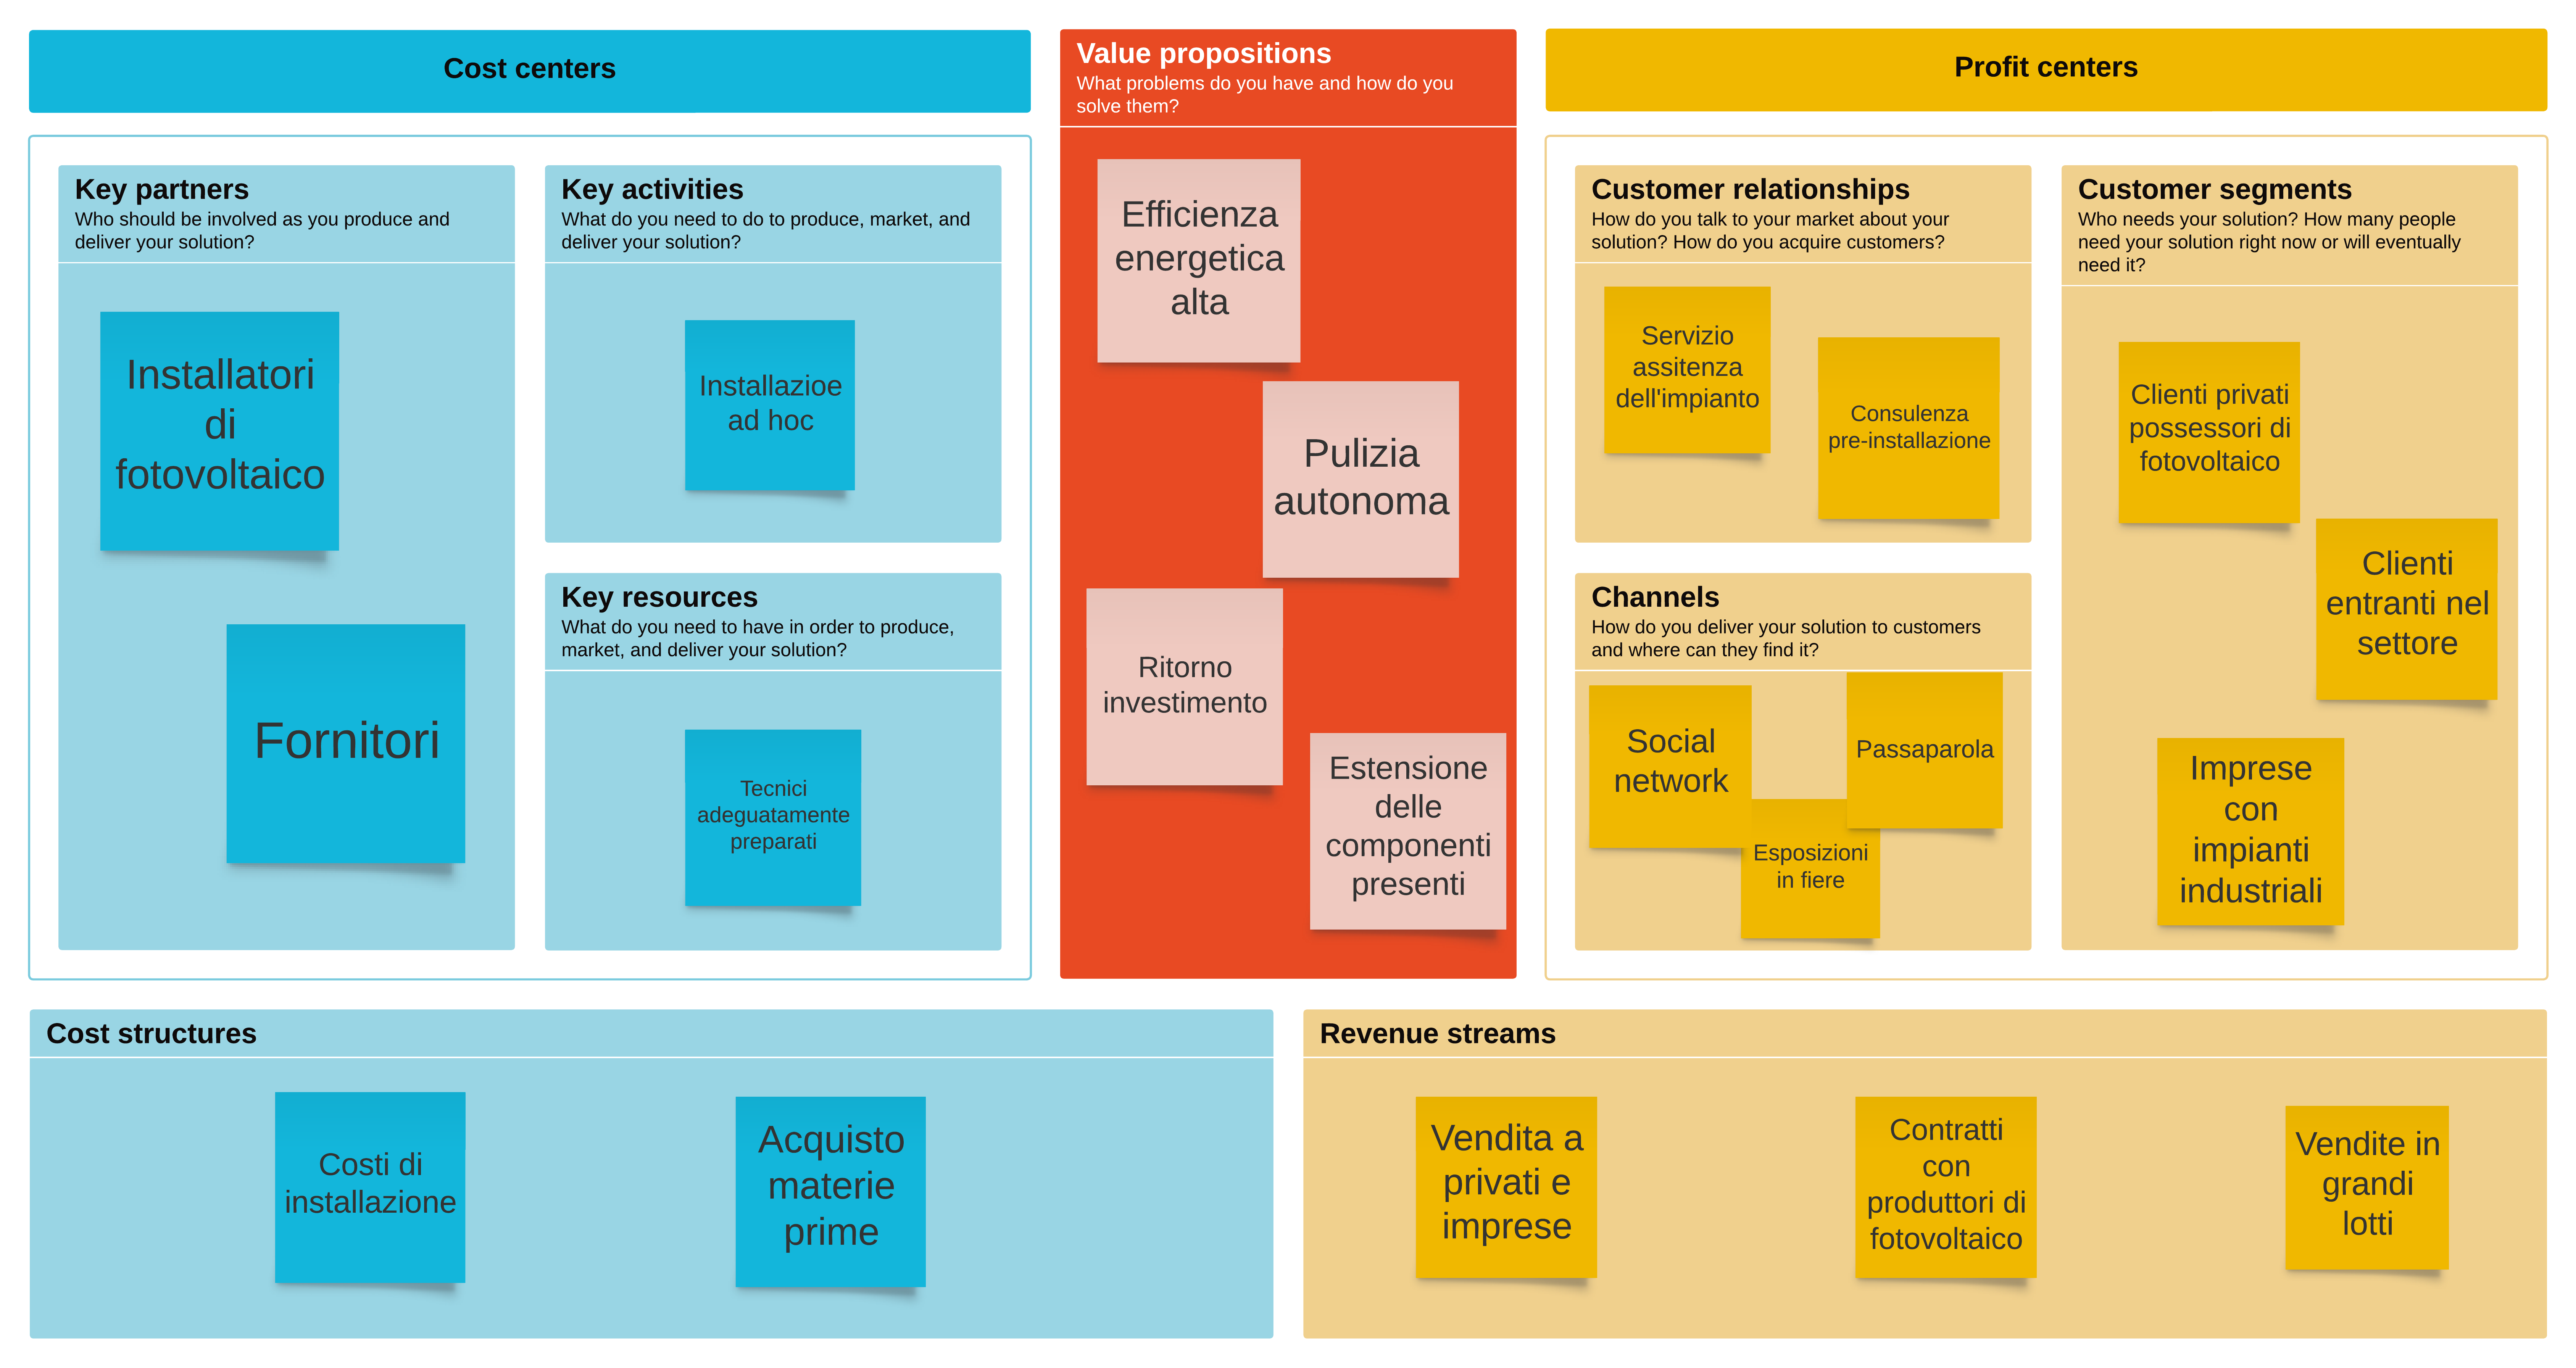
\includegraphics[width=\textwidth]{Images/BusinessModelCanvas.png}
	% idee:
	%	- esprimere il costo di una tradizionale pulizia, il nostro prodotto avrà un costo circa pari a quello della singola pulizia ma consentirà al cliente di non pacgare più per altri interventi
	%	- costi: manodopera per installazione (dipende da installazione a installazione) e materie prime... diciamo un 50 euro + manodopera?
	%	- prezzo di vendita = costi + 25%?
	\section{Funzionamento del prodotto}
	%cosa dire:
	% descrizione introduttiva delle funzionalita offerte dalla soluzione 
	\emph{Osmos} è un sistema di supporto alla pulizia di un impianto fotovoltaico principalmente composto da un device in grado di monitorare l'efficienza dei pannelli 
	e un supporto idraulico per il rilascio del detergente sul pannello. \'E inoltre dotato di un recipiente sufficientemente ampio per poter contenere l'acqua osmotica necessaria ad almeno un lavaggio.\\
	\begin{wrapfloat}{figure}{r}{0pt}
		\includegraphics[width=0.5\textwidth]{Images/PROTOTIPO3.JPG}
	\end{wrapfloat}
	Il device principale che gestisce l'intera logica della pulizia, si compone di un microcontrollore in grado di monitorare l'efficienza energetica dei pannelli. Ciò avviene intercettando tramite rete wireless i report prodotti dagli ottimizzatori installati nell'impianto fotovoltaico. Ogniqualvolta questi producono un report, le informazioni raccolte vengono mantenute all'interno del device di \emph{Osmos} in modo da tener traccia di uno storico dello stato recente dell'impianto (indicativamente gli ultimi 15 giorni).\\
	Il microcontrollore è alimentato a batteria facilmente sostituibile esternamente, senza dover entrare in contatto con le componenti elettroniche, ed inoltre è accessoriato con un display e un'interfaccia a led che mostrano l'efficienza dell'impianto:
	\begin{itemize}
		\item sul display viene riportato il valore percentuale dell'efficienza energetica letta dall'ultimo report;
		\item l'interfaccia luminosa è invece composta da 3 led (rosso, giallo e verde) in modo che il led illuminato sia rappresentativo delle condizioni di pulizia del pannello.
	\end{itemize}
	Si stabiliscono quindi due soglie, configurabili dal cliente, A (consigliata del 90\%) e B (consigliata dell'85\%) tali che:
	\begin{itemize}
		\item se il valore dell'efficienza E è superiore alla soglia A ($E \ge A$) allora viene acceso il led verde;
		\item se il valore dell'efficienza E è compreso tra la soglia B e A ($B \le E < A$) allora viene acceso il led giallo;
		\item se il valore dell'efficienza E è inferiore alla soglia B ($E < B$) allora viene acceso il led rosso;
	\end{itemize}
	L'accensione del led rosso innesca anche l'avvio della pulizia automatica di \emph{Osmos}.\\\\
	% QUI METTEREI GRAFICO CON ANDAMENTO DELL'EFFICIENZA (a gradini)
	Sebbene il prodotto sia pensato per una minima interazione col cliente, è comunque reso disponibile un interruttore manuale, attivabile dall'esterno, per innescare il meccanismo di pulizia in qualunque momento.\\
	All'avvio della procedura di pulizia, il microcontrollore attiva un sistema idraulico che rilascia l'acqua osmotica sul pannello tramite un getto a media pressione.\\\\
	% descrizione del sistema idraulico
	Il supporto idraulico del sistema è composto da una pompa idraulica e un serbatoio contenente il detergente. Al momento della pulizia la pompa idraulica viene attivata per scaricare, tramite un apposito sportello l'acqua osmotica sulla superficie fotovoltaica. Il detergente esausto viene smaltito dal sistema nella rete idraulica dell'edificio.
	Il sistema prevede un facile accesso al serbatoio in modo da facilitare le operazioni di carico del detergente, in modo che l'utente sia in grado di riempirlo nuovamente in autonomia.
	% MONSTER ALLERGY MI FAN STARNUTIR
	% quali tecnologie gia esistenti sfrutta la soluzione
	\section{WBS e prospetto di Gantt}
	In precedenza sono stati elencati gli elementi e attività fondamentali per \emph{Osmos}. Questi possono essere pianificati racchiudendoli in 4 macro attività (\emph{Work Packages}) che rappresentano l'intero progetto:
	\begin{enumerate}
		\item \textbf{Project management}\\
			  L'insieme delle attività riguardanti la pianificazione stessa, la gestione delle risorse e lo studio dell'ambito dell'impresa tramite analisi del settore e analisi del mercato. L'output di questo \emph{work package} è un documento contenente tutti i dati necessari e ad ottimizzare il lavoro successivo, come delle adeguate conoscenze del segmento di mercato selezionato oppure lo schedule dei lavori successivi.
		\item \textbf{Prototipazione}\\
			  Le attività che hanno come output finale la realizzazione di un MVP specifico, da mostrare ad investitori ed \emph{early adopters} in grado di rendere l'idea di ciò che sarà il prodotto finale, implementando solo quelle caratteristiche per cui il cliente è disposto a pagare: la gestione automatica della pulizia e il monitoraggio dell'efficienza. L'MVP consentirà di testare e validare le idee del prodotto senza spreco economico e temporale nella realizzazione del prodotto completo.
		\item \textbf{Produzione}\\
			  Superate le prime fasi di vita dell'impresa, \emph{Osmos} dovrà occuparsi della vera e propria realizzazione dei prodotti completi. Questo \emph{work package} raccoglie quindi le attività di ottenimento delle materie prime e costruzione, assemblaggio vero e proprio, del prodotto finito.
		\item \textbf{Commercializzazione}\\
			  Ultimo insieme di attività che può anche essere eseguito parzialmente in parallelo col precedente. Rappresenta principalmente il rapporto col cliente e la diretta vendita del prodotto.
	\end{enumerate}
	Di seguito è riportata la struttura delle WBS nel dettaglio:
	\begin{center}
		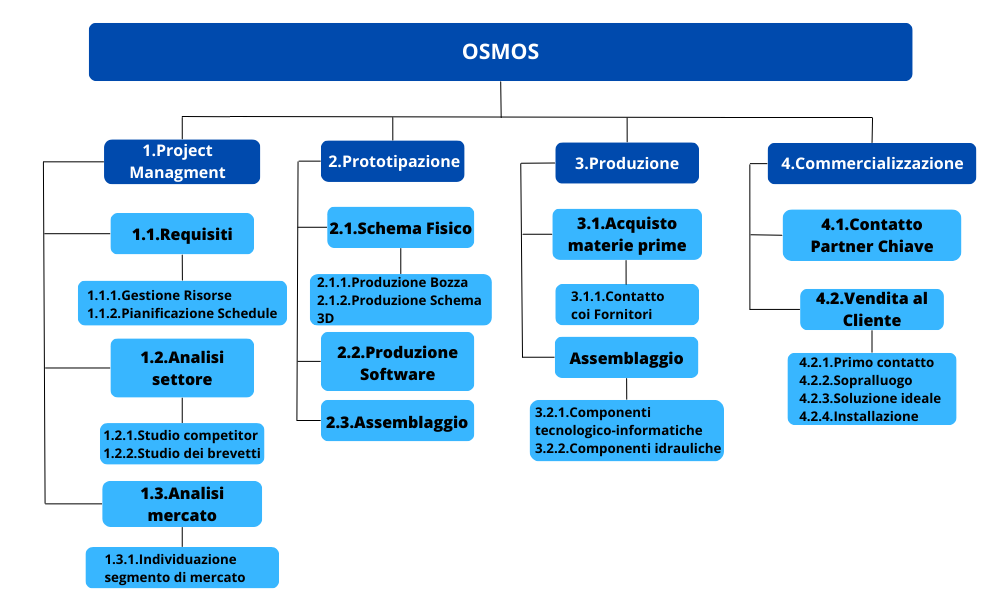
\includegraphics[width=\textwidth]{Images/WBS.png}
	\end{center}
	Ad ogni singola WBS che è riportata in questa struttura gerarchica sono associati vincoli temporali per il loro completamento. Le diverse attività sono inoltre assegnati a 3 diversi team operativi:
	\begin{itemize}
		\item Team A $\rightarrow$ si occupa sia della fase di pianificazione sia della parte organizzativa legata alla gestione delle risorse materiali e non;
		\item Team B $\rightarrow$ dedicato inizialmente alla realizzazione del prototipo, successivamente avrà il compito di occuparsi dell'assemblaggio dei prodotti finiti prima della consegna al cliente;
		\item Team C $\rightarrow$ il cui compito sarà relazionarsi col cliente presentandogli personalmente il prodotto, individuando la soluzione più adatta a lui e procedendo con l'installazione a domicilio.
	\end{itemize}
	Gli obiettivi temporali sono riportati nel seguente diagramma di Gantt. Per completezza, un diagramma maggiormente dettagliato è presente in appendice.
	\begin{center}
		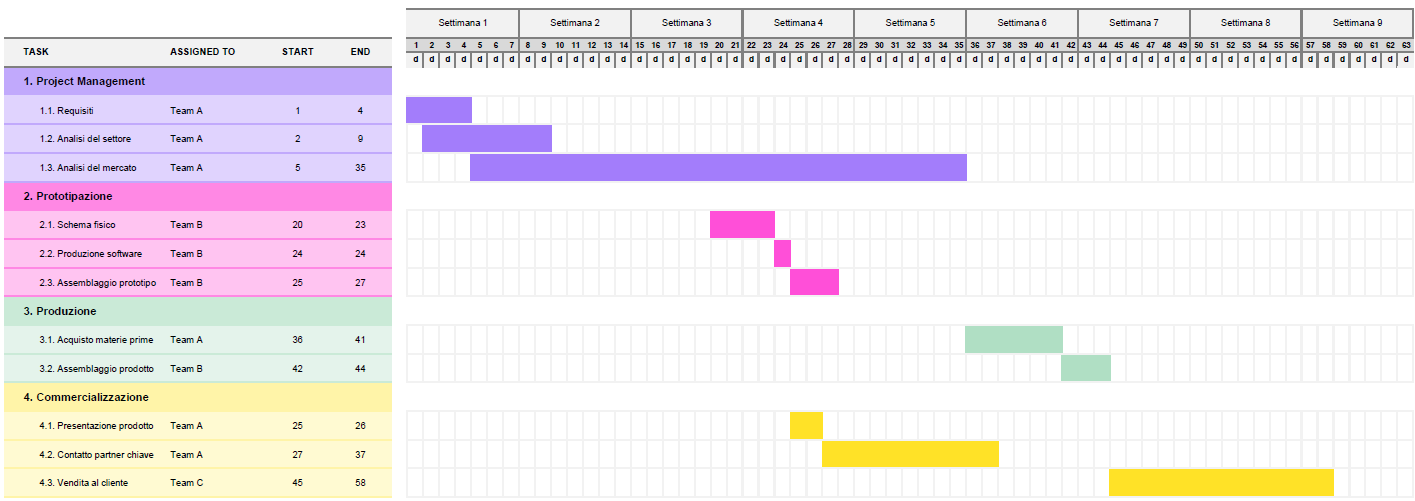
\includegraphics[width=\textwidth]{Images/gantt.png}
	\end{center}
	\newpage
	\section{Appendice}
	Elemento \#1 - Prospetto di Gantt completo
	\begin{center}
		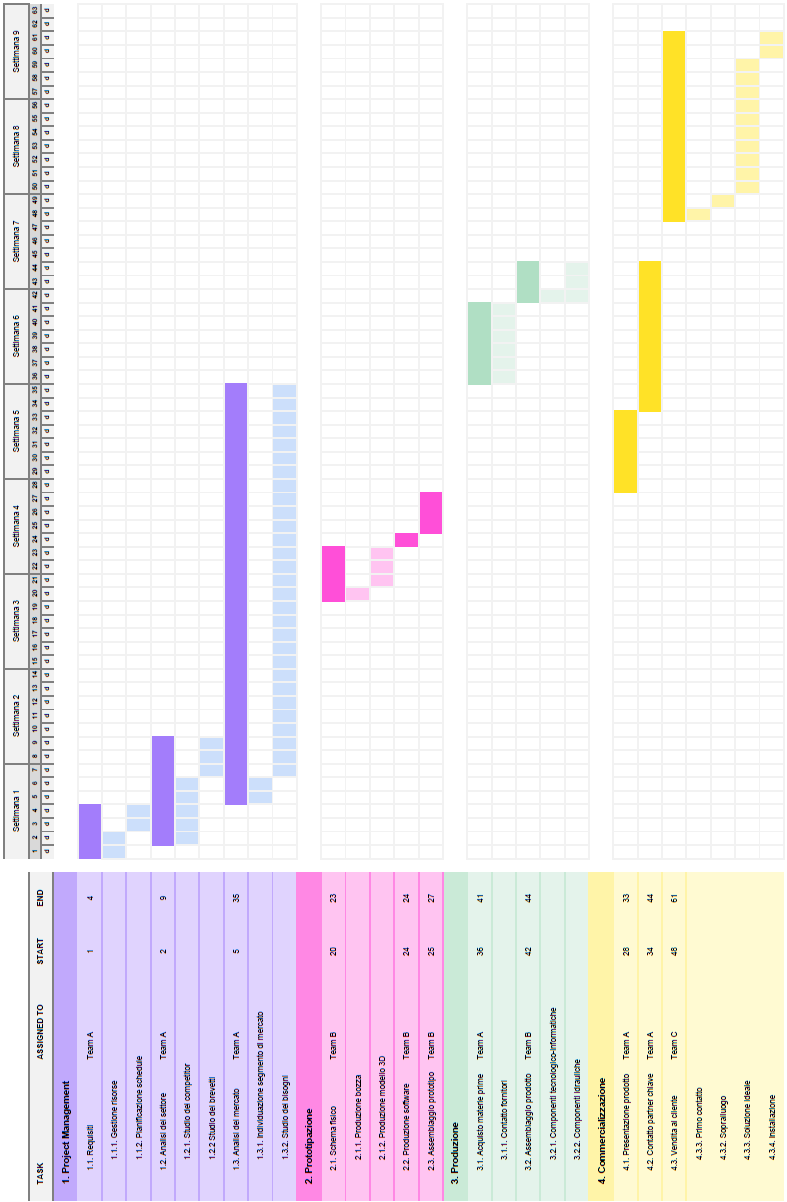
\includegraphics[width=0.9\textwidth]{Images/gantt_full.png}
	\end{center}
\end{document} 
